\chapter{Debugging and Profiling} \label{debugging}
%====================================
\index{debugger}
\index{tracing|(}
\section{Prolog-style Tracing and Debugging}
%===========================
\index{tracing!Prolog Programs}
%
XSB supports a version of the Byrd four-port debugger for interactive
debugging and tracing of Prolog code.  In this release (\version), it
does not work very well when debugging code involving tabled
predicates~\footnote{The current version of XSB's Prolog debugger does
  not include exceptions as a debugging port.}.  If one only creeps
(see below), the tracing can provide some useful information.  For
programs that involve large amounts of tabling forest-view tracing can
be used (Section~\ref{sec:forest-trace}).
To turn on tracing, use {\tt trace/0}, {\tt trace/1}, or {\tt trace/2}.  To
turn tracing off, use {\tt notrace/0}.

\begin{description}
\repeatstandarditem{trace}{trace/0}
\standarditem{notrace}{notrace/0}

When tracing is on, the system will print a message each time a
predicate is:
\begin{enumerate} \index{debugger!ports}
\item initially entered (Call), 
\item successfully returned from (Exit), 
\item failed back into (Redo), and
\item completely failed out of (Fail).  
\end{enumerate}
When debugging interactively, a message may be printed and tracer
stopped and prompts for input.  (See the predicates {\tt show/1} and
{\tt leash/1} described below to modify what is traced and when the
user is prompted.)

In addition to single-step tracing, the user can set spy points to
influence how the tracing/debugging works.  A spy point is set using
{\tt spy/1}.  Spy points can be used to cause the system to enter the
tracer when a particular predicate is entered. Also the tracer allows
``leaping'' from spy point to spy point during the debugging process.
%
The debugger also has profiling capabilities, which can measure the cpu
time spent in each call. The cpu time is measured only down to 0.0001-th
of a second.

When the tracer prompts for input, the user may enter a return, or a single
character followed by a return, with the following meanings:
\bi
\index{trace!options}
\item{\tt c, <CR>}: {\em Creep}~ Causes the system to single-step to
  the next port (i.e.\ either the entry to a traced predicate called
  by the executed clause, or the success or failure exit from that
  clause).
\item{\tt a}: {\em Abort}~ \index{abort!trace facility} Causes execution to abort
  and control to return to the top level interpreter.
\index{break level}
\item{\tt b}: {\em Break}~ Calls the evaluable predicate {\em break},
  thus invoking recursively a new incarnation of the system
  interpreter.  The command prompt at break level $n$ is
  \begin{center}
    {\tt $n$: \tt ?-}
  \end{center}
  The user may return to the previous break level by entering the system
  end-of-file character (e.g.\ {\tt ctrl-D}), or typing in the atom 
  {\tt end\_of\_file}; or to the top level interpreter by typing in
  {\tt abort}.
\item{\tt f}: {\em Fail}~ Causes execution to fail, thus transferring
  control to the Fail port of the current execution.
\item{\tt h}: {\em Help}~ Displays the table of debugging options.
\item{\tt l}: {\em Leap}~ Causes the system to resume running the
  program, only stopping when a spy-point is reached or the program
  terminates.  This allows the user to follow the execution at a
  higher level than exhaustive tracing.
\item{\tt n}: {\em Nodebug}~ Turns off debug mode.
\item{\tt r}: {\em Retry (fail)}~ Transfers to the Call port of the current
  goal.  Note, however, that side effects, such as database modifications
  etc., are not undone.
\item{\tt s}: {\em Skip}~ Causes tracing to be turned off for the entire
  execution of the procedure.  Thus, nothing is seen until control comes
  back to that procedure, either at the Success or the Failure port.
\item{\tt q}: {\em Quasi-skip} This is like Skip except that it does not mask
  out spy points.
\item{\tt S}: {\em Verbose skip}~ Similar to {\tt Skip} mode, but trace
  continues to be printed. The user is prompted again when the current call
  terminates with success or failure.  This can be used to obtain a full
  trace to the point where an error occurred or for code profiling. (See
  more about profiling below.)
\item{\tt e}: {\em Exit}~ Causes immediate exit from \ourprolog\ back to the
  operating system.
\ei
%/* TLS: it seems like there may not be much use for the non-queryable trace/1 */

\standarditem{trace(+Filename,+option)}{trace/2}
\index{trace!logging}
%\index[pred]{\texttt{trace/1}}
%\index{\texttt{trace/1}}
%
{\tt trace/2} is like {\tt trace/0} except that it is non-interactive
and dumps trace information into a log file, {\tt Filename}.
Currently the only supported option is \texttt{log}.  However, the log
is written in the form of Prolog facts, which can be loaded
queried. The format of the facts is:
%% 
\begin{verbatim}
xsb_tracelog(CallId,CallNum,PortType,ParentCallNum,DepthOfCall,CurrentCall,Time)
\end{verbatim}
%% 
where \texttt{CallId} is an identifier generated when XSB encounters a
new top-level call. This identifier remains the same for all subgoals
called while tracing that top-level call.
\bi
\item \texttt{CallNum} is a generated number to show the nesting of
  the calls being traced. It is the same number that the user sees
  when tracing interactively.
%
\item \texttt{PortType} is \texttt{'Call'}, \texttt{'Redo'},
  \texttt{'Exit'}, or \texttt{'Fail'}.  
\item \texttt{ParentCallNum} is the call number of the parent call.
%
\item \texttt{DepthOfCall} is the nesting depth of the current call
  with respect to its ancestor calls.  
%
\item \texttt{CurrentCall} is the call being traced
%
\item \texttt{Time} is the CPU time it took to execute
  \texttt{CurrentCall}. On \texttt{'Call'} and \texttt{'Redo'},
  \texttt{Time} is always 0 --- it has a meaningful value only for the
  \texttt{'Exit'} and \texttt{'Fail'} log entries. 
\end{itemize}
It should be noted that when calls are delayed due to the well-founded
negation computation of because of the \texttt{when/2} primitive, the
parent call might be off in some cases. However, the parent property
repairs itself for subsequent calls.

`The name of the predicate (\texttt{xsb\_tracelog}) used for logging
can be changed by asserting it into the predicate
\texttt{debug\_tracelog\_predicate/1}, which should be imported from
\texttt{usermod}. For instance,
%% 
\begin{verbatim}
   :- import debug_tracelog_predicate/1 from usermod.
   ?- assert(debug_tracelog_predicate(foobar)).
\end{verbatim}
%% 

\standarditem{spy(Preds)}{spy/1}
    where {\tt Preds} is a spy specification or a list of such
    specifications, and must be instantiated. This predicate sets spy
    points (conditional or unconditional) on predicates.  A spy
    specification can be of several forms. Most simply, it is a term
    of the form $P$/$N$, where $P$ is a predicate name and $N$ its
    arity.  Optionally, only a predicate name can be provided, in
    which case it refers to all predicates of any arity currently
    defined in {\tt usermod}.  It may optionally be prefixed by a
    module name, e.g.  $ModName$:$P$/$N$. (Again, if the arity is
    omitted, the specification refers to all predicates of any arity
    with the given name currently defined in the given module.)  A spy
    specification may also indicate a conditional spy point. A
    conditional spy specification is a Prolog rule, the head
    indicating the predicate to spy, and the body indicating
    conditions under which to spy. For example, to spy the predicate
    p/2 when the first argument is not a variable, one would write:
    $spy (p(X,\_):-nonvar(X)).$ (Notice that the parentheses around
    the rule are necessary). The body may be empty, i.e., the rule may
    just be a fact.  The head of a rule may also be prefixed (using
    $:$) with a module name. One should not put both conditional and
    unconditional spy points on the same predicate.

\standarditem{nospy(Preds)}{nospy/1}
    where {\tt Preds} is a spy specification, or a list of such
    specifications, and must be instantiated at the time of call.  What
    constitutes a spy specification is described above under {\tt spy}.
    {\tt nospy} removes spy points on the specified predicates. If a
    specification is given in the form of a fact, all conditional spy points
    whose heads match that fact are removed.

\standarditem{debug}{debug/0}
    Turns on debugging mode.
    This causes subsequent execution of predicates with trace or spy
    points to be traced, and is a no-op if there are no such predicates.
    The predicates {\tt trace/0}, {\tt trace/1}, \texttt{trace/2},  and {\tt spy/1} cause debugging mode
    to be turned on automatically.

\standarditem{nodebug}{nodebug/0}
    Turns off debugging mode.  This causes trace and spy points to be ignored.

\standarditem{debugging}{debugging/0}
    Displays information about whether debug mode is on or not, and lists
    predicates that have trace points or spy points set on them.

\standarditem{debug\_ctl(option,value)}{debug\_ctl/2}
   {\tt debug\_ctl/2} performs debugger control functions as described below.
   These commands can be entered before starting a trace or inside the trace.
   The latter can be done by responding with ``{\tt b}'' at the prompt,
   which recursively invokes an XSB sub-session. At this point, you can
   enter the debugger control commands and type \verb|end_of_file.| This
   returns XSB back to the debugger prompt, but with new settings.
   %%
   \begin{enumerate}
   \item {\tt debug\_ctl(prompt, off)} Set non-interactive mode globally.
     This means that trace will be printed from start to end, and the user
     will never be prompted during the trace.
    \item {\tt debug\_ctl(prompt, on)} 
      Make tracing/spying interactive.
    \item {\tt debug\_ctl(profile, on)}  
      Turns profiling on. This means that each time a call execution
      reaches the {\tt Fail} or {\tt Exit} port, CPU time spent in that
      call will be printed. The actual call can be identified by locating a
      {\tt Call}  prompt that has the same number as the ``cpu time''
      message.
    \item {\tt debug\_ctl(profile, off)}  
      Turns profiling off.
    \item {\tt debug\_ctl(redirect, +File)} 
      Redirects debugging output to a file. This also includes program output,
      errors and warnings.
      Note that usually you cannot see the contents of {\tt +File} until it
      is closed, {\it i.e.}, until another redirect operation is performed
      (usually {\tt debug\_ctl(redirect, tty)}, see next).
    \item {\tt debug\_ctl(redirect, tty)}     
      Attaches the previously redirected debugging, error, program output,
      and warning streams back to the user terminal.
    \item {\tt debug\_ctl(show, +PortList)}  
      Allows the user to specify at which ports should trace messages be
      printed. {\tt PortList} must be a list of port names, i.e., a sublist
      of ['Call', 'Exit', 'Redo', 'Fail']. 
    \item {\tt debug\_ctl(leash, +PortList)}  
      Allows the user to specify at which ports the tracer should stop
      and prompt the user for direction.  {\tt PortList} must be a list of
      port names, i.e., a sublist of ['Call', 'Exit', 'Redo', 'Fail'].  Only
      ports that are {\tt show}-n can be {\tt leash}-ed. 
    \item {\tt debug\_ctl(hide, +PredArityPairList)}  
      The list must be of the form {\tt [P1/A1, P2/A2, ...]}, {\it i.e.},
      each either must specify a predicate-arity pair. Each predicate on
      the list will become non-traceable. That is, during the trace, each
      such predicate will be treated as an black-box procedure, and trace
      will not go into it.
    \item {\tt debug\_ctl(unhide, ?PredArityPairList)} If the list is a
      predicate-arity list, every predicate on that list will become
      traceable again. Items in the list can contain variables. For
      instance, {\tt debug\_ctl(unhide, [\_/2])} will make all 2-ary that
      were previously made untraceable traceable again.  As a special case,
      if {\tt PredArityPairList} is a variable, all predicates previously
      placed on the ``untraceable''-list will be taken off.
    \item {\tt debug\_ctl(hidden, -List)}
      This returns the list of predicates that the user said should not be
      traced.
   \end{enumerate}
   %%
\end{description}


\subsection{Control of Prolog-Style Tracing and Debugging}
%--------------------------------------------------
\index{tracing!Prolog Program!Controls}
%
\index{low-level tracing} \index{tracing!low-level}

XSB debugger also provides means for the low-level control of what
must be traced. Normally, various standard predicates are masked out
from the trace, since these predicates do not make sense to the
application programmer.  However, if tracing below the application
level is needed, you can retract some of the facts specified in the
file {\tt syslib/debugger\_data.P} (and in some cases assert into
them). All these predicates are documented in the header of that
file. Here we only mention the four predicates that an XSB developer
is more likely to need. To get more trace, you should retract from the
first three predicates and assert into the last one.
%%
\begin{itemize}
\item {\tt hide\_this\_show(Pred,Arity)}: specifies calls (predicate name and
  arity) that the debugger should {\tt not} show at the prompt. However,
  the evaluation of this hidden call {\tt is} traced.
\item {\tt hide\_this\_hide(Pred,Arity)}: specifies calls to hide. Trace
  remains off while evaluating those predicates. Once trace is off, there
  is no way to resume it until the hidden predicate exits or fails.
\item  {\tt show\_this\_hide(Pred,Arity)}: calls to show at the
  prompt. However, trace is switched off right after that.
\item  {\tt trace\_standard\_predicate(Pred,Arity)}: Normally trace doesn't
  go inside standard predicates ({\it i.e.}, those specified in
  {\tt syslib/std\_xsb.P}. If you need to trace some of those, you must
  {\tt assert} into this predicate.
\end{itemize}
%%
In principle, by retracting all facts from the first three predicates and
asserting enough facts into the last one, it is possible to achieve the
behavior that approximates the {\tt -T} option. However, unlike {\tt -T},
debugging can be done interactively. This does not obviate {\tt -T},
however. First, it is easier to use {\tt -T} than to issue multiple asserts
and retracts. Second, {\tt -T} can be used when the error occurs early on,
before the moment when XSB shows its first prompt.

Finally, XSB also provides a facility for low-level tracing of Prolog
execution.  This can be activated by invoking the emulator with the
{\tt -T} option (see Section~\ref{sec:EmuOptions}), or through the
predicate {\tt trace/0}.  \stdrefindex{\$trace/0} It causes trace
information to be printed out at {\em every} Prolog call (including
those to system predicates, and tabled predicates).  While this method
can occasionally be useful, its use is limited.  For tabled executions
the techniques in the following sections are much more appropriate.
Ever for Prolog programs, the volume of such trace information can become
very large very quickly, so this method of tracing is only recommended
for situations where no other debugging method is useful.

%-----------------------------------------------------------------------------
\newcommand{\ctrace}{{\tt logforest}}

\section{Trace-based Execution Analysis through Forest Logging} \label{sec:forest-trace}
%
The tracing and debugging described in previous sections has proven
useful for Prolog programs for 30 or more years.  However, when
tabling is added to Prolog, things change.  First, as described in
Chapter~\ref{chap:TablingOverview}, tabling can be used to find the
least fixed point of mutually recursive predicates.  Operationally,
this requires the ability to suspend one computation path and to
resume another.  Second, the addition of tabled negation for the
well-founded semantics requires the ability to delay negative goals
whose only proof may be involved in a loop through negation and to
simplify these goals once their truth value has become
known. Furthermore, a tabled subgoal has different states: it may be
{\em new}; it may be {\em incomplete} so that new answers might be
derived for it; or {\em completed} (completely evaluated) so that the
answers may simply be read from the table.  In short, tabling, which
can execute much more general programs than Prolog and which can use
the stronger well-founded semantics, requires a more complex set of
operations than Prolog's SLDNF.  Accordingsly, debugging and tracing
is correspondingly more complex.  Thus, while Prolog's 4-port debugger
may be useful for programs that involve just a few tabled predicates,
it may not be useful for programs that heavily use tabling for complex
recursions, non-monotinic reasoning or other purposes.

There is currently no standard approach to debugging tabled programs.
One possible approach would be to extend the 4-port debugger to
include other ports for tabling operations.  Such extensions have not
yet been explored, and whether the paradigm of n-port debugging can be
extended to full tabling so that it can be useful to programmers is an
open question.  Another approach would be use the declarative approach
of {\em justification} \cite{GuRR01,PGDRR04} to explain why
derivations were or were not made.  XSB does in fact have a
justification package but it is not currently robust enough to be
recommended for general use.  Below we present the {\tt \ctrace}
approach~\cite{Swif14b}

\subsection{Tracing a tabled evaluation through forest logging}
%
While the operations used for tabling are more complex than those of
SLDNF, they have a clear formal operational semantics through SLG and
the forest-of-trees model.  We recall this model briefly below for a
definite program but assume a background knowledge of tabled logic
programming (see, for instance~\cite{SwiW12}).

\begin{example} \rm 
Figure~\ref{fig:local} shows a program fragment along with an SLG
forest for the query {\tt ?- reach(1,Y)} to the the right-recursive
tabled predicate {\tt reach/1}.  An SLG forest consists of an SLG tree
for each tabled subgoal $S$: this tree has root $S \mif{} S$.  In a
definite program an SLG tree represents resolution of program clauses
and answers to prove $S$.  In Figure~\ref{fig:local} each non-root
node of the form $K. N$ where $N = (S \mif{} Goals)\theta$ is a clause
in which the bindings to a subgoal $S$ are maintained in $S\theta$,
the goals remaining to prove $S$ are in $Goals\theta$, and the order
of creation of $N$ within the tabled evaluation is represented by a
number, $K$ (local scheduling is used in this example).  Children of a
root node are obtained through resolution of a tabled subgoal against
program clauses.  Children of non-root nodes are obtained through
answer clause resolution, if the left most selected literal is tabled
(e.g. children of node 3 or 11 in the tree for {\tt reach(1,Y)}), or
through program clause resolution if the leftmost selected literal is
not tabled (e.g. children of nodes 2 and 18 in the tree for {\tt
  reach(1,Y)}).  Nodes that have empty {\em Goals} are termed {\em
  answers}.
%
\begin{figure}[htbp]
\centering
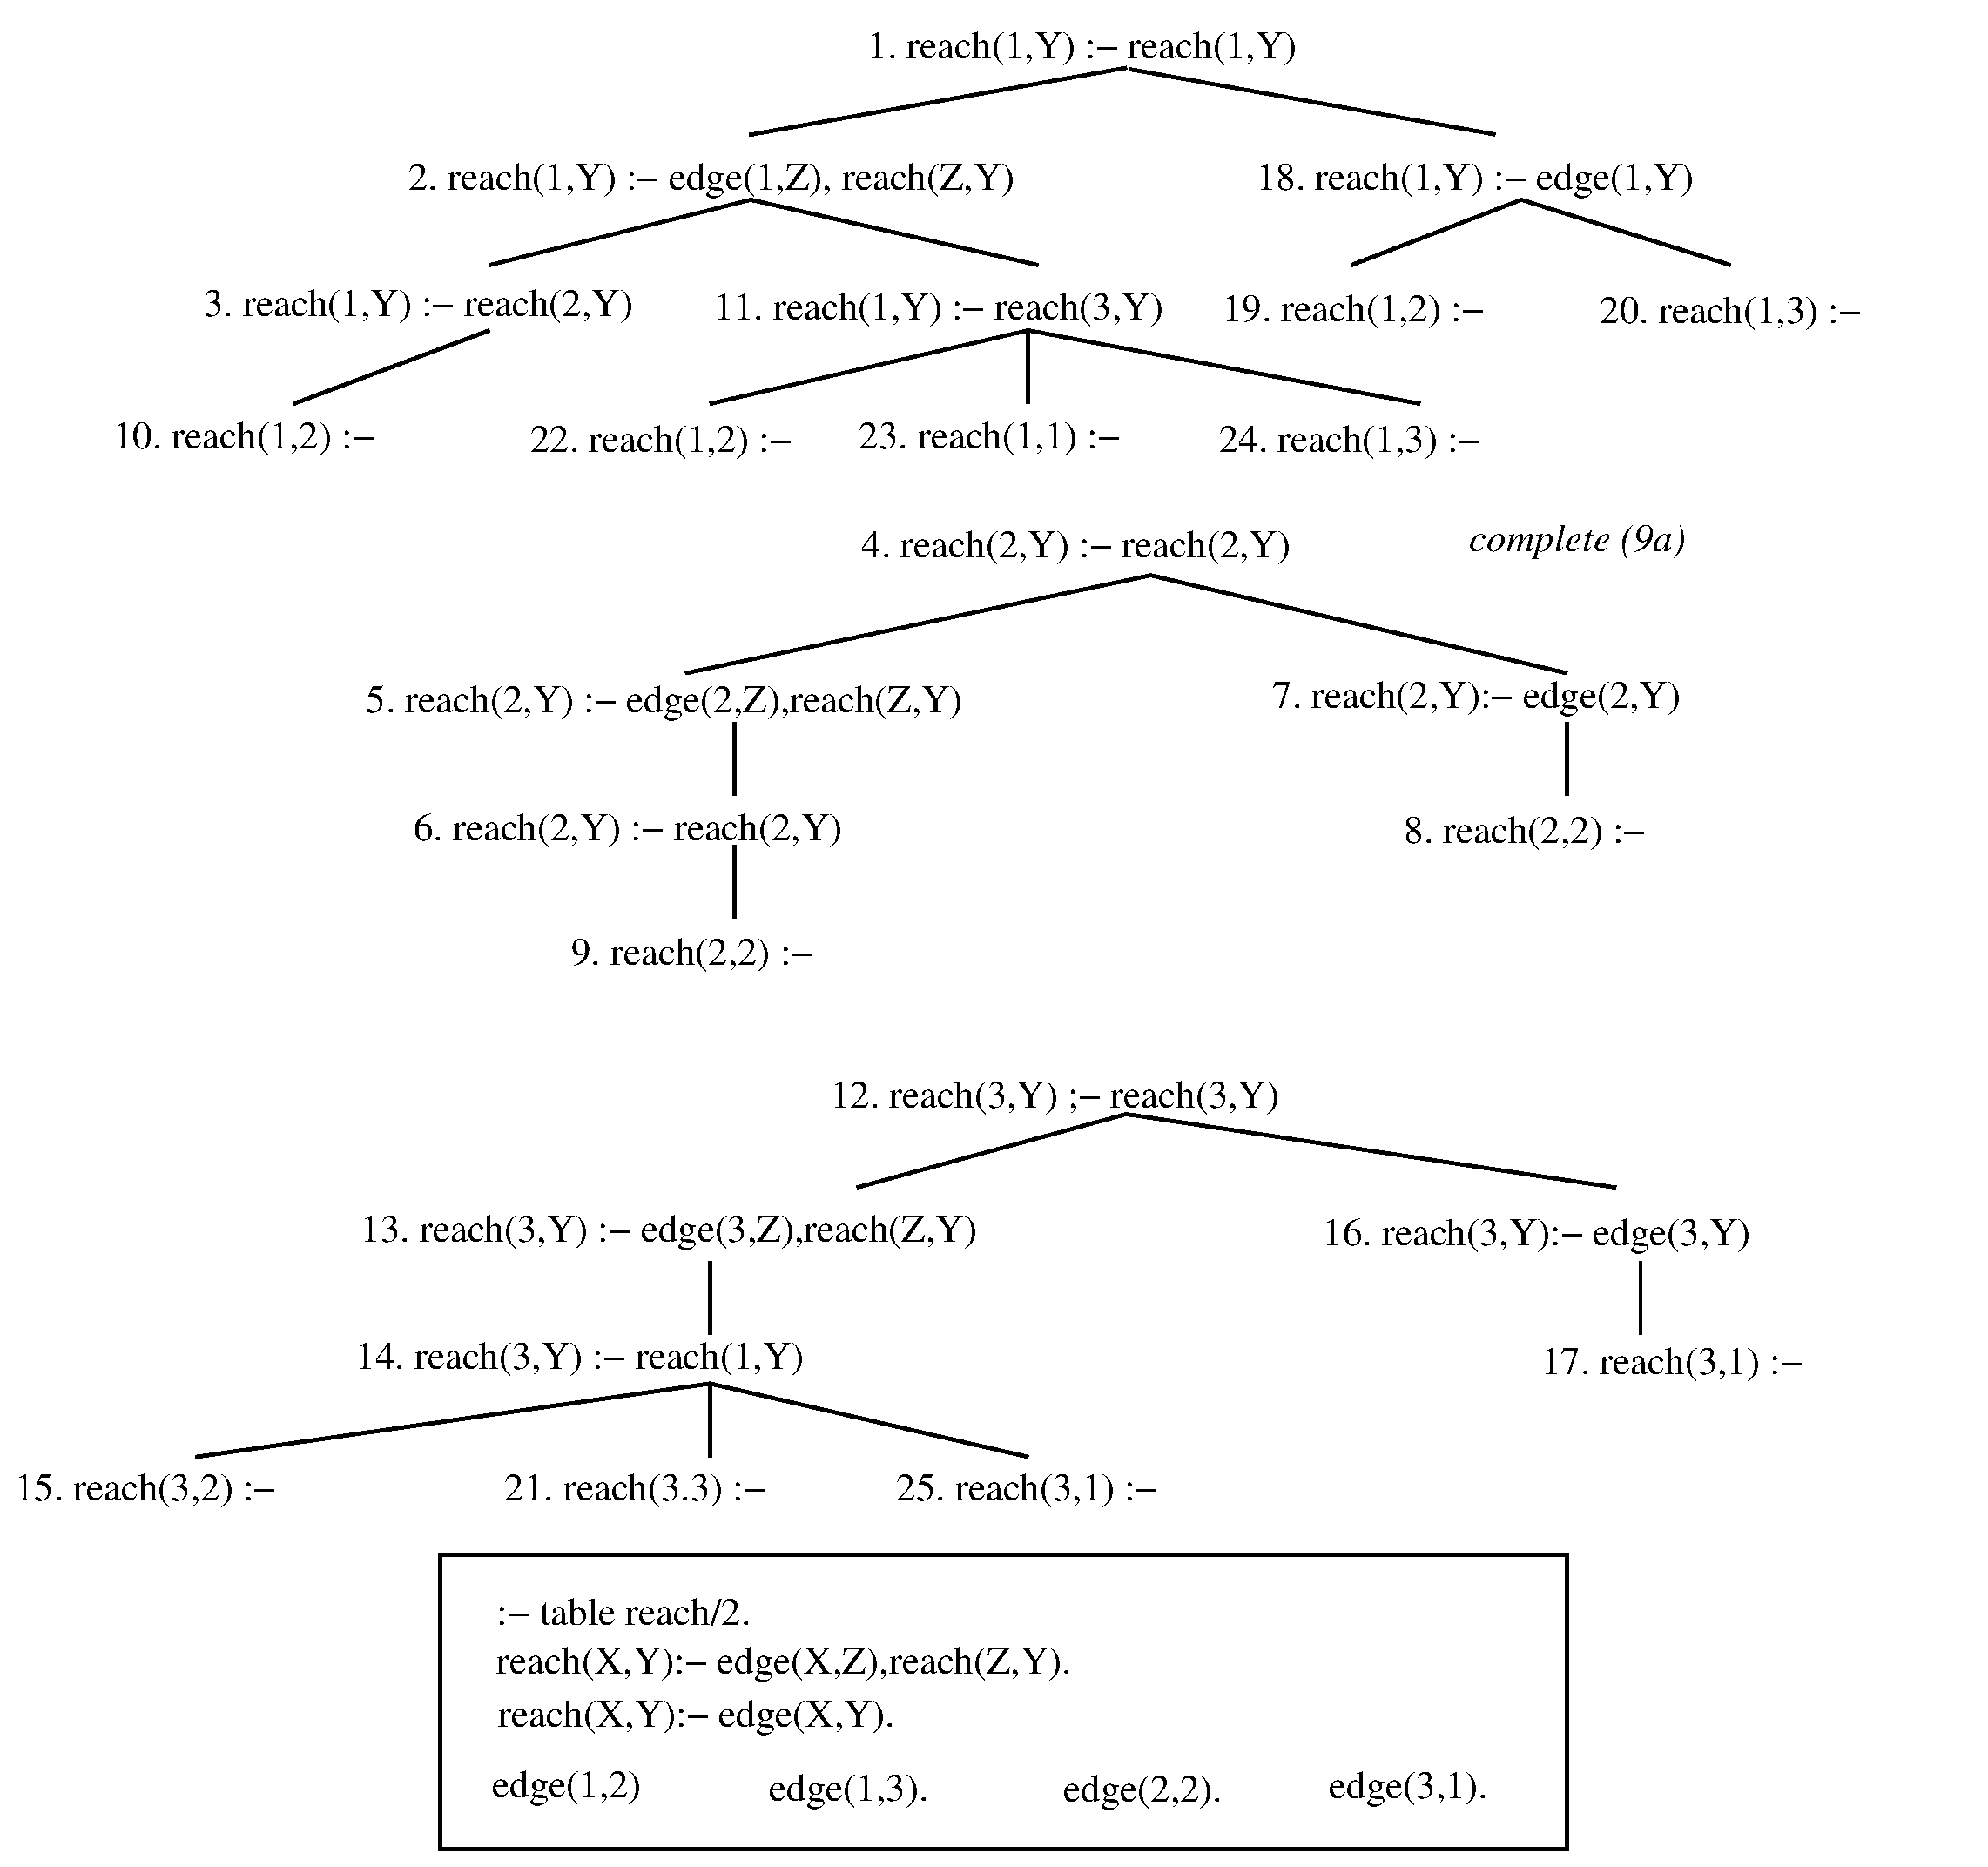
\includegraphics[width=.99\textwidth]{slg-forest-local}
%%\mbox{
%%{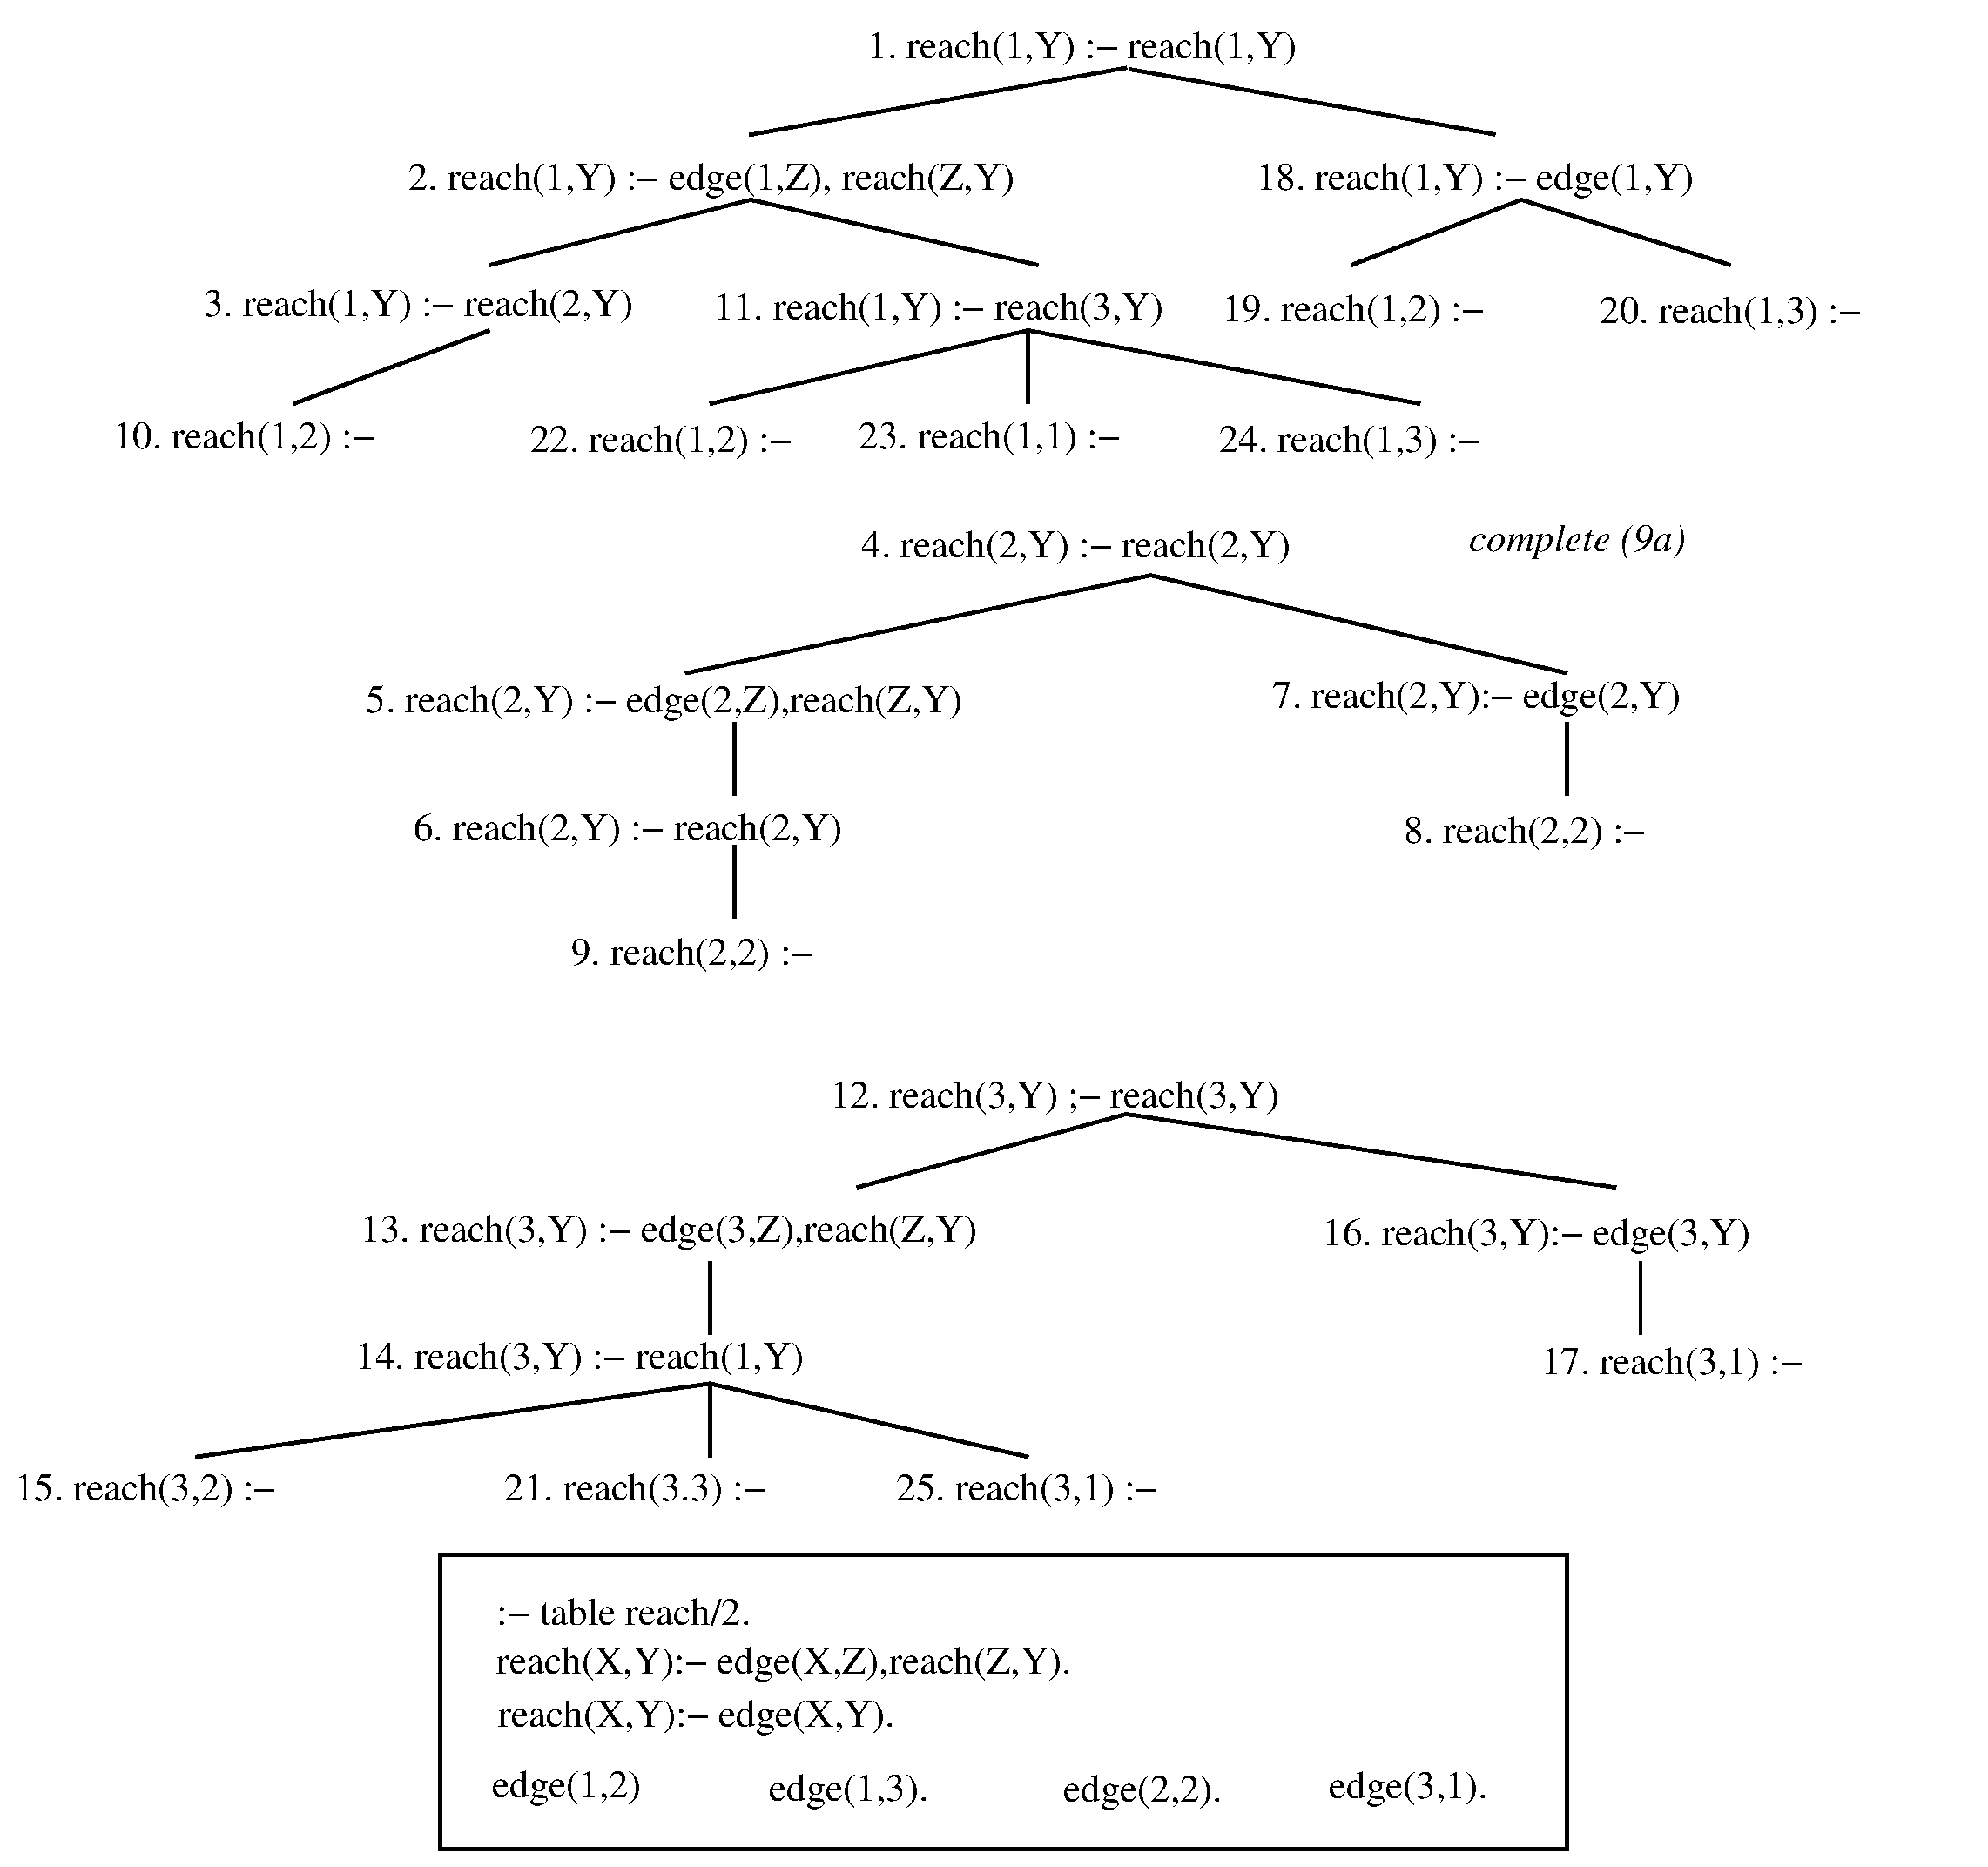
\epsfig{file=slg-forest-local,width=.99\textwidth}}}
\caption{A program $P_{Rrec}$ and SLG forest for (local) evaluation of
  {\tt ?- reach(1,Y)}} \label{fig:local}
\end{figure}
%
Note that the evaluation keeps track of each tabled subgoal $S$ that
it encounters.  Later if $S$ is selected again, resolution will use
answers rather than program clauses; if no answers are available, the
computation will {\em suspend} at that point and the evaluation will
backtrack to try to derive answers using some other computation path.
Once more answers have been derived, the evaluation {\em resumes} the
suspended computation.  Similarly, once the computation has
backtracked through all answers available for $S$ in the current
state, the computation path will suspend, and resume after further
answers are found.  Thus a tabled evaluation is a fixed point
computation for a set of interdependent subgoals.  When it is
etermined that a (perhaps singleton) set of subgoals can produce no
more answers, the subgoals are completed.
\end{example}

%\vspace{0.1in}

The forest logging approach ({\tt \ctrace}) allows one to run a tabled
query and produce a log that can be interpreted as (a partial image
of) an SLG forest.  The log can then used to analyze program
correctness, to optimize performance and so on.  Because \ctrace{}
  produces a log, it superficially resembles the non-interactive trace
  described earlier in this chapter.  However,
\begin{itemize}
\item {\tt trace/1} produces a Prolog-style trace that takes little
  account of tabling.  \ctrace{} structures its output according to
  the forest-of-trees model, and takes little account of program
  clause resolution.

\item \ctrace{} is implemented in C for efficiency, while {\tt
  trace/1} is built on top of XSBs interactive debugger.  Unlike {\tt
  trace/1}, \ctrace{} can therefore to produce logs for very large
  evaluations with little overhead.
\end{itemize}

Currently, \ctrace{} captures the following actions.

\bi
\item {\em A call to a tabled subgoal}~ If a positive call to a tabled
  subgoal $S_1$ is made from a tree for $S_2$ a Prolog-readable fact
  of the form {\tt tc(S1,S2,Stage,Counter)} is logged, where {\em
    Counter} is the ordinal number of the fact, and {\tt Stage} is
\bi
\item {\tt new} if $S_1$ is a new subgoal
\item {\tt cmp} if $S_1$ is not a new subgoal and has been completed
\item {\tt incmp} if $S_1$ is not a new subgoal but has {\em not} been
  completed 
\ei 
%
If the call is negative a fact of the form {\tt
  nc(S1,S2,Stage,Counter)} is logged, where all arguments are as
above.

  For instance, in the above example, node 3 would be represented as
  {\tt tc(reach(2,Y),reach(1,Y),2)} (the reason for using the counter
  value of 2 rather than 3 is explained below).  If $S_1$ is the first
  tabled subgoal in an evaluation, $S_2$ is the atom {\em null}.

\item {\em Derivation of a new answer}~ When a new {\em unconditional}
  answer $A$ is derived for subgoal $S$ and added to the table
  (i.e. $A$ is not already an answer for $S$) a fact of the form {\tt
    na(A,S,Counter)} is logged.  In the above example, the answer node
  9 would be represented as {\tt na([2],reach(2,\_v1),4)} where the
  first argument is a list of substitutions for the variables {\em
    \_v1,...,\_vn} in $S$.

  When a new {\em conditional} answer $A \mif D|$, with substitution
  $A$ and delayed literals $D$. is derived for subgoal $S$ and added
  to the table a fact of the form {\tt nda(A,S,D,Counter)} is logged.

\item {\em Return of an answer to a consuming subgoal}~When an
  unconditional answer $A$ is returned to a consuming subgoal $S$ in a
  tree for $S_T$, a fact of the form {\tt ar(A,S,ST,Counter)} is
  logged.  A log entry is made only if the table for $S$ is incomplete
  (see the explanation below).

  If the answer $A$ is conditional, the fact has the form {\tt
    dar(A,S,ST,Counter)}, where each argument is as above.

\item {\em Delaying a selected negative literal}.  If a selected
  negative literal $L$ of a node $N$ is delayed, because it is
  involved in a loop through negation, and $N$ is in a tree for $S_T$,
  a fact of the form {\tt dly(L,$S_T$,Counter)} is logged.

\index{strongly connected components (SCCs)}
\item {\em Subgoal completion}
\bi
\item When a set $\cS$ of subgoals is determined to be completely
  evaluated and is completed, a fact of the form {\tt
    cmp(S,SCCNum,Counter)} is logged for each $S \in \cS$.  Here
  $SCCNum$ is simply a number giving an ordinal value that can be used
  to group subgoals into mutually dependent sets of subgoals (here
  called {\em Strongly Conneced Components} or {\em SCCs}), i.e. the
  {\em SCCNum} of each $S \in \cS$ has the same value, but that value
  is not used for a completion fact of any subgoal not in $\cS$.
%
\index{tabling!early completion of subgoals}
\item When a subgoal $\cS$ is {\em early completed}, i.e. it is
  determined that no more answers for $S$ are possile or are desired a
  fact of the form {\tt cmp(S,ec,Counter)} is logged.  If $S$ belonged
  to a larger mutually dependent set $\cS$ when it was early
  completed, $S$ will also be included in the completion facts for
  $\cS$.
\ei
\item {\em Table Abolishes}
\bi
\item When a tabled subgoal $S$ is abolished, a fact of the form {\tt
  ta(subg(S),Counter)} is logged.
\item When all tables for a predicate $p/n$ are abolished, a fact of
  the form {\tt ta(pred(p/n),Counter)} is logged.
\item When all tables are abolished, a fact of the form {\tt ta(all,Counter)} is logged.
\ei
%
\item {\em Location of errors} Whenever an error is thrown and the
  execution is in a tree for a subgoal $S$, a Prolog-readable fact of
  the form {\tt err(S,Counter)} is logged, where {\em Counter} is the
  ordinal number of the fact.  The primary purpose of this fact is to
  indicate the nearest tabled call that gave rise to an uncaughterror.  \ei

{\tt logforest} does {\em not} contain

\bi
\item Information about the occurrence of program clause resolution
  either when used to produce children of tabled predicates, or when
  it is used to produce children whose nodes have a selected literal
  that is non-tabled.

\item Information about the return of answers from completed tables.
  XSB uses a so-called {\em completed table optimization} which treats
  answer return from completed tables in a manner akin to program
  clause resolution.  
 \ei

\index{attributed variables}
\noindent
The inclusion of the above two features in {\tt logforest} would
significantly slow down execution of XSB.  However, future versions of
{\tt logforest} may include expanded logging features for negation,
for call and answer subsumption and for incremental
tabling~\footnote{Currently, attributes of attributed variables are
  not printed out.}.

\begin{example}
The forest for {\tt reach(1,Y)} in the foregoing example has the log
file as shown in Table~\ref{tab:fview}.

\begin{table}[htbp]
\begin{tabular}{lll}               \\ \hline  
Log File                                     & Forest & Explanation\\ \hline 
tc(reach( 1,\_v0),null,new,0)                & node 1 & \\
                                             & node 2 & created by program clause resol. \\
                                             & node 3 & created by program clause resol. \\
tc(reach( 2,\_v0),reach( 1,\_v0),new,1)      & node 4 & \\
                                             & node 5 & created by program clause resol.\\
                                             & node 6 & created by program clause resol. \\
tc(reach( 2,\_v0),reach( 2,\_v0),incmp,2)    &        & repeated subgoal registered\\
                                             & node 7 & created by program clause resol. \\
                                             & node 8 & created by program clause resol. \\
na([ 2],reach( 2,\_v0),3)                    & node 8 & registered as answer\\
ar([ 2],reach( 2,\_v0),reach( 2,\_v0),4)     & node 9 & created by answer resol.\\
cmp(reach( 2,\_v0),2,5)                      &    9a   & {\tt reach(2,\_v0)} completed \\
                                             & node 10 & created by return from completed table \\
na([ 2],reach( 1,\_v0),6)                    & node 10 & registered as an answer\\
                                             & node 11 & created by program clause resol. \\
tc(reach( 3,\_v0),reach( 1,\_v0),new,7)      & node 12 & \\
                                             & node 13 & created by program clause resol. \\
                                             & node 14 & created by program clause resol. \\
tc(reach( 1,\_v0),reach( 3,\_v0),incmp,8)    & node 14 & repeated subgoal registered \\
ar([ 2],reach( 1,\_v0),reach( 3,\_v0),9)     & node 15 & created by answer resol. \\
na([ 2],reach( 3,\_v0),10)                   & node 15 & registered as an answer \\
                                             & node 16 & created by program clause resol. \\
                                             & node 17 & created by program clause resol. \\
na([ 1],reach( 3,\_v0),11)                   & node 17 & registered as an answer \\
                                             & node 18 & created by program clause resol. \\
                                             & node 19 & created by program clause resol. (repeated answer)\\
                                             & node 20 & created by program clause resol.\\
na([ 3],reach( 1,\_v0),12)                   & node 20 & registered as an answer\\
ar([ 3],reach( 1,\_v0),reach( 3,\_v0),13)    & node 21 & created by answer return\\
na([ 3],reach( 3,\_v0),14)                   & node 21 & registered as an answer\\
ar([ 2],reach( 3,\_v0),reach( 1,\_v0),15)    & node 22 & created by answer resol.\\
ar([ 1],reach( 3,\_v0),reach( 1,\_v0),16)    & node 23 & created by answer resol.\\
na([ 1],reach( 1,\_v0),17)                   & node 23 & registered as an answer \\
ar([ 3],reach( 3,\_v0),reach( 1,\_v0),18)    & node 24 & created by answer resol. \\
ar([ 1],reach( 1,\_v0),reach( 3,\_v0),19)    & node 25 & created by answer resol.v \\
cmp(reach( 1,\_v0),1,20)                     &  & \\
cmp(reach( 3,\_v0),1,21)   & & \\ \hline
\end{tabular}
\caption{Log file for computation in Figure~\ref{fig:local}}\label{tab:fview}
\end{table}
\end{example}

\begin{description}
\ourrepeatmoditem{log\_forest(+Call)}{log\_forest/2}{tables}
\ourmoditem{log\_forest(+Call,+Options)}{log\_forest/2}{tables}
%
These predicates turn on forest logging, call {\tt Call}, then turn
logging off when {\tt Call} is finished.  {\tt Options} is a list of
possible options.
%
\bi
\item If {\tt Options} contains the term {\tt file(File)} then direct
  the logging to {\tt File}; otherwise the log will be sent to
  standard output.
\item If {\tt Options} contains the term {\tt level(Level)} where {\tt
  Level} = {\tt full} or {\tt partial} then the level of forest
  logging is set to the respective value.  The default level is {\tt
    full}.  The level {\tt partial} does not output answer return
  operations, and so can reduce the size of the log for certain
  computations.  The actions of partial logging and full logging are
  otherwise the same.  \ei
%  Currently, the only option is
%   {\tt file(File)}, which directs the logging to the file {\tt File}.
%   If {\tt Options} is an empty list or if {\tt log\_forest/1} is
%   called, the log will be sent to standard output~\footnote{Future
%     options will be able to turn on and off the logging of various
%     types of facts.}.

{\bf Error Cases} 
\bi
\item {\tt Options} is a variable, or contains a variable as an element
\bi
\item {\tt instantiation\_error}
\ei
\item {\tt Options} is not a list
\bi
\item {\tt type\_error(list,Options)}
\ei
\item {\tt Options} contains an option {\tt O} that is not a forest
  logging option.  
\bi
\item {\tt domain\_error(forest\_logging\_option,O)}
\ei
\ei


\index{indexing}
\ourmoditem{load\_forest\_log(+File)}{load\_forest\_log/1}{tables}
%
The log produced by {\tt log\_forest/[1,2]} is a Prolog file that can
be compiled and/or loaded dynamically just as any other Prolog file.
However, for large logs (i.e. those of many megabytes) use of {\tt
  load\_dync/[1,2]} XSB commands can drastically reduce the time
needed to load the file, while use of the proper {\tt index/2}
declarations can greately improve query time.  The simple predicate,
{\tt load\_forest\_log/1} loads a log file and indexes needed arguments.
\end{description}

\index{tracing|)}

\subsection{Analyzing the log; seeing the forest through the trees} \label{sec:forest-log-anal}
%
As previously described, forest logging is based on the formal
operational semantics of SLG, and as a result the log can be analyzed
to query any result that can be modelled by the theory.  But despite
the power of forest logging, it can be difficult to use.  Not all
users have the background to fully understand the operational
semantics of SLG.  Even those users with a formal background may find
it difficult to write efficient analysis routines for logs of large
computations~\footnote{I find it difficult myself!}.  Accordingly, XSB
provides routines that analyze logs and display information about a
computation.  These routines can answer many questions about a
computation and can provide the starting point for further
exploration.  We introduce these routines via an extended example.

\begin{example} \rm \label{ex:scc-anal}
%
This example arises from the actual use of forest logging to
understand a Flora-2 computation~\cite{YaKZ05}, in which the Cyc
reasoner (cf. http://www.cyc.com) was translated into Silk
(cf. http://silk.semwebcentral.org) and used to answer various
questions in biology.  Silk itself compiles into Flora-2 which in turn
compiles into XSB~\footnote{This example was run in 2012 using a
  64-bit server with a large amount of RAM.}.  After translation,
query answering took more resources than expected, and users wanted to
determine why.  Using the features of \version{}, the first step is to
call {\tt statistics/0} at the end of the computation.  The statistics
indicated that the computation took about 30 seconds of CPU time and
300 megabytes of table space, while XSB's trail had allocated over 1
gigabyte of space.  The call to {\tt statistics/0} also showed the
following information:
%
\begin{verbatim}
  8678944 variant call check/insert ops: 615067 producers, 8063877 variants.
  317346 answer check/insert ops: 304899 unique inserts, 12447 redundant.
\end{verbatim}
In other words, there were nearly 10 million tabled subgoals that were
called, indicating that this computation was heavily tabled (a
characteristic of most Flora-2 computations), It also shows that the
average number of answers per tabled subgoal is rather small.

This basic information leads to several questions.  Why were there so
many tabled subgoals?  Did the tabling have anything to do with the
large amount of choice-point/trail space that was allocated?  Which
tabled subgoals had answers?  How many times did a given tabled
predicate call another tabled predicate?

\index{\texttt{table\_dump/2}}\index{\texttt{table\_dump/3}} Some of
these questions can be answered by {\tt table\_dump/[2,3]}:
particularly, what tabled subgoals were called, and which had answers.
However {\tt table\_dump/[2,3]} cannot provide other information, such
as the dependencies of given tabled subgoals on other tabled subgoals
or the order in which operations occurred.  From a formal perspective,
{\tt table\_dump/[2,3]} does not allow a user to analyze an entire SLG
forest: only the ``table'', i.e., the subgoals in the forest and the
unordered set of its answers.  The table omits any information about
interior nodes or completion information, both of which are used to
compute dependency information.  Dependencies are useful in analyzing
most computations, but is especially important in Flora-2 computations
such as this one, that make heavy use of HiLog.  This use of HiLog
means that the dependencies of tabled predicates on one another is not
at all obvious, and may not easily be determined by static analysis.

The next step, therefore, in analyzing this computation is to rerun it
with forest logging.  For this computation forest logging has no
impact on memory usage, but increases the time of the computation from
about 30 seconds to about 52 seconds --- around 73\% in this case.  It
is worthwhile noting that the actual overhead of forest logging varies
depending on how heavily the computation is tabled.  The log itself
had slightly over 14 million entries which were loaded into XSB via
{\tt load\_forest\_log/1}.  The log took about 140 seconds to load and
about 7.8 Gbytes of space for the log facts and their multiple and
trie indexes~\footnote{The load time for this example, about 100,000
  facts/second is typical for 2012 CPUs; the size of the loaded code
  is larger than usual, due in part to the expansion in the size of
  terms caused by the HiLog encoding.}.

The easiest way to start the analysis is to ask the query {\tt ?-
  forest\_log\_overview}, which for this example gives:
%
\begin{verbatim}
There were 613496 subgoals in 463330 (completed) SCCs.  
93918 subgoals were early-completed.  
0 subgoals were not completed in the log.
There were a total of 8670043 tabled subgoal calls:
    613496 were calls to new subgoals
    4467747 were calls to incomplete subgoals
    3588800 were calls to complete subgoals

Number of SCCs with 1 subgoals is 463322
Number of SCCs with 4 subgoals is 1
Number of SCCs with 7 subgoals is 1
Number of SCCs with 52 subgoals is 1
Number of SCCs with 110 subgoals is 4
Number of SCCs with 149671 subgoals is 1
\end{verbatim}
%
\index{tabling!complete evaluation}
\index{tabling!early completion of subgoals} 
%
The overview extends the information shown by {\tt
  statistics/0}.  First, the total number of completed and
non-completed SCCs is given along with a count of how many of the
completed subgoals were early completed.  Information about
non-completed SCCs is useful, since the forest log may be analyzed for
a computation that does not terminate.  Since this computation did
terminate, all subgoals in the log were completed~\footnote{The slight
  difference between the number of subgoals shown here and the number
  shown by {\tt statistics/0} is due to the use of tabling in the
  Flora compiler.}.  Note that there is also a breakdown of calls to
tabled subgoals that distinguishes whether the tabled subgoal was new,
completed, or incomplete.  Recall that calls to completed tabled
subgoals essentialy treat the answers in the table as facts, so that
these calls are efficient.  Making a call to an incomplete subgoals on
the other hand means that the calling and called subgoals are mutually
recursive~\footnote{This statement is true in local evaluation but not
  in batched evaluation.} and execution of recursive sets of subgoals
can be expensive, especially in terms of space.

Finally, the overview report provides the distributions of tabled
subgoals across SCCs.  While most of the SCCs were small there was a
large one, with nearly 150,000 mutually dependent subgoals.  Clearly
the large SCC should be examimed.  The first step is to obtain its
index.  The query
%
\begin{verbatim}
get_scc_size(SCC,Index)), Index > 1000.
\end{verbatim}
%
returns the information that the index of the large SCC was 39.  The
query {\tt analyze\_an\_scc(39,userout)} then provides the following
information.
%
\begin{verbatim}
There are 149671 subgoals and 4461290 links (average of 30.8073 edges per subgoal) 
      within the SCC

There are 2 subgoals in the SCC for the predicate backchainForbidden / 0
There are 2 subgoals in the SCC for the predicate 
                   http://www.cyc.com/silk/implementation/transformationPredicate / 0
:
There are 15613 subgoals in the SCC for the predicate gpLookupSentence / 3
There are 15613 subgoals in the SCC for the predicate removalSentence / 3
There are 18770 subgoals in the SCC for the predicate forwardSentence / 3
There are 18771 subgoals in the SCC for the predicate lookupSentence / 3

Calls from assertedSentence/3 to lookupSentence/3 : 32
Calls from backchainForbidden/0 to 'http://www.cyc.com/silk/implementation/transformationPredicate'/0 : 2
:
Calls from transformationSentence/2 to sbhlSentence/3 : 5479
Calls from tvaSentence/3 to removalSentence/3 : 7695
\end{verbatim}
%
It is evident from the first line in this report that the vast
majority of the calls to incomplete tables during this computation
occur in the SCC under investigation.  Since information on incomplete
tables is kept in XSB's choice point stack (cf. \cite{SaSw98}), the
evaluation of SCC 39 is the likely culprit behind the large amount of
stack space required.  The subgoals in the SCC are first broken out by
their predicate name and arity, then the edges within the SCC are
broken out by the predicates of their caller and called subgoals.  At
this point a programmer can review the various rules for {\tt
  lookupSentence/3}, {\tt forwardSentence/3} and other predicates to
determine whether the recursion is intended and if so, whether it can
be simplified.
%
\end{example}

\subsubsection{Using abstraction in the analysis}
%
Within the SCC analysis, information about a given tabled subgoal $S$
was abstracted to the functor and arity of $S$.  For this example,
abstraction was necessary, as reporting 150,000 subgoals or 4,000,000+
would not provide useful information for a human being.  However, it
could be the case that seeing the tabled subgoals themselves would be
useful for a smaller SCC.  Even for an SCC of this size, different
levels of abstraction could be useful: mode information or type
information might be useful in a given circumstance.  

\begin{example} \label{ex:moded-scc-anal} \rm
%
Making the call {\tt ?-
  analyze\_an\_scc(39,userout,abstract\_modes(\_,\_))} applies the
predicate {\tt abstract\_modes/2} to each term, producing an output of
the form:
%
\begin{verbatim}
There are 149671 subgoals and 4461290 links (average of 30.8073 edges per subgoal) 
           within the SCC

There are 3 subgoals in the SCC for the predicate backchainRequired(g,g)
There are 2 subgoals in the SCC for the predicate backchainForbidden(g,g)
:
There are 29254 subgoals in the SCC for the predicate gpLookupSentence(g,g)
There are 29254 subgoals in the SCC for the predicate removalSentence(g,g)

Calls from assertedSentence(g,g) to lookupSentence(g,g) : 10
Calls from assertedSentence(m,g) to lookupSentence(m,g) : 22
:
Calls from transformationSentence(m,g) to sbhlSentence(m,g) : 741
Calls from tvaSentence(g,g) to removalSentence(g,g) : 7695
\end{verbatim}
%
{\tt abstract\_modes(In,Out)} simply goes through each argument of
{\tt In} and unifies the corresponding argument of {\tt Out} with a
{\tt v} if the argument is a variable, a {\tt g} if the argument is
ground, and {\tt m} otherwise.  

\end{example}
%
{\tt abstract\_modes/2} is simply an example: any term-abstraction
predicate may be passed into the last argument of {\tt
  analyze\_an\_scc/3}~\footnote{Because of the special representation
  of Flora-2 terms, abstraction was used to produce the output of
  Example~\ref{ex:moded-scc-anal}, while a more sophisticated version
  of {\tt abstract\_modes/2} was used in
  Example~\ref{ex:moded-scc-anal}.}.

\subsubsection{Analyzing Negation}
%
Many programs that use negation are stratified in such a way that they
do not require the use of {\sc Delaying} and {\sc Simplification}
operations, and the routines described in the previous section are
sufficient for these programs.  However if a program does not have a
two-valued well-founded model, a user would often like to understand
why.  Even in a program that is two-valued, the heavy use of {\sc
  Delaying} and {\sc Simplification} can indicate that some rules may
need to be optimized by having their literals reordered.

\begin{example} \label{ex:neg} \rm
Figure~\ref{fig:neg} shows a program with negation and illustrates SLG
resolution for the query {\em p(c)} to the program.  The nodes in
Figure~\ref{fig:neg} have been annotated with the order in which they
were created under local scheduling. In the formalism used by
Figure~\ref{fig:neg}, the symbol $|$ in a node separates the
unresolved goals to the right from the delayed goals to the left.  In
the evaluation state where nodes 1 through 10 have been created, {\em
  p(b)} has been completed, and {\em p(a)} and {\em p(c)} are in the
same SCC.  There are no more clauses or answers to resolve, but {\em
  p(a)} is involved in a loop through negation in node 5, and nodes 2
and 10 involve {\em p(a)} and {\em p(c)} in a negative
loop~\footnote{In this example, we ignore the effects of early
  completion which would complete {\em p(b)} immediately upon creation
  of node 8, obviating the need to create node 9.}.

In situations such as this, where all resolution has been performed
for nodes in an SCC, an evaluation may have to apply a {\sc Delaying}
operation to a negative literal such as {\em not(p(a))}, in order to
explore whether other literals to its right might fail. 
% In cases such as this, 
When multiple literals can be delayed, an arbitrary one is chosen to
be delayed first.  So the evaluation delays the selected literal of
node 2 to generate node 12 producing a {\em conditional answer} -- an
answer with a non-empty delay list
(cf. Section~\ref{sec:conditional-answers} for an overview of how XSB
computes and allows inspection of delayed literals).  Next, {\em not
  p(a)} in node 5 is delayed, failing that computation path, and {\em
  not p(c)} in node 10 is delayed to produce node 15 and failing the
final computation path for {\em p(a)}.  At this stage the SCC
$\{p(a),p(c)\}$ is {\em completely evaluated} meaning that there are
no more operations applicable for goal literals (as opposed to delay
literals).  Since {\em p(a)} is completely evaluated with no answers,
conditional or otherwise, the evaluation determines it to be {\em
  failed} and a {\sc Simplification} operation can be applied to the
conditional answer of node 12, leading to the {\em unconditional}
answer in node 17 and {\em success} of the literal {\em p(c)}.
\end{example}

\begin{figure*}[tbp] 
\begin{center}
%\fbox{\epsfig{file=Figures/del-simpl3.eps,width=\textwidth}}
\epsfig{file=del-simpl3.eps,width=\textwidth}
\end{center}
\caption{A Normal Program and SLG Forest for Evaluation of the Query {\em p(c)}}
\label{fig:neg}
\end{figure*}


As indicated previously, the forest log overview includes a total
count of {\sc Delaying} and {\sc Simplification} operations, as well
as a count of conditional answers.  In addition, SCC analysis counts
negative as well as positive links within the SCC.  The current
version of forest logging also provides a means to examine the causes
of answers that have an undefined truth value.  Recall from
Example~\ref{ex:neg} that there are two types of causes of an
undefined truth value: either 1) a negative literal explicitly
undergoes a {\sc Delaying} operation; or 2) a conditional answer may
be used to resolve a literal.  It can be shown that in local
evaluation, a conditional answer $A$ will never be returned out of an
SCC if $A$ is successful or failed in the well-founded model of a
program.  This means that if an answer for $S$ is undefined, then it
would be caused operationally by a {\sc Delaying} operation within the
SCC of $S$ or within some other SCC on which $S$ depends.  So to
understand why an atom is undefined it can be useful understand the
``root causes'' of the delay: to examine SCCs in which {\sc Delaying}
operations were executed and conditional answers were derived, but the
answers could not be simplified.
% into unconditional answers.

\begin{example}
As a use case, logging was made of execution of a Flora-2 program that
tested out a new defeasibility theory.  The forest log overview
indicated that the top-level query was undefined: 
%
\begin{small}
\begin{verbatim}
:
There were a total of 55 negative delays
There were a total of 0 simplifications
There were a total of 695 unconditional answers derived:
There were a total of 66 conditional answers derived:
\end{verbatim}
\end{small}
%
The analysis predicate {\tt three\_valued\_scc(List)} produces a list
of all SCC indices in which {\sc Delaying} caused the derivation of
conditional answers.  These SCCs can then be analyzed as discussed in
the previous section.
\end{example}

\subsection{Discussion}
%
Using log forest imposes a relatively minimal overhead on most
computations, considering the information it can provide, and loading
and analysis is relatively quick.  For this example, the top level
analysis took around 10 seconds, and analysing SCC 39 took about 20
seconds in Example~\ref{ex:scc-anal} and about 60 seconds in
Example~\ref{ex:moded-scc-anal}.  For more information,
see~\cite{Swif14b}.

\subsection{Predicates for Forest Logging}

\begin{description}
\ourmoditem{forest\_log\_overview}{forest\_log\_overview/0}{tables}
%
Provides an overview of subgoals, calls, and SCCs in the forest log as
indicated in Section~\ref{sec:forest-log-anal}.

\ourmoditem{get\_scc\_size(?Index,?Size)}{get\_scc\_size/3}{tables}
%
This simple predicate determines the indices of SCCs whose size is
{\tt Size}, for use with {\tt analyze\_an\_scc/[2,3]}.

\ourmoditem{three\_valued\_sccs(List)}{three\_valued\_scc/1}{tables}
%
If there are any SCCs in the log where delay is performed, causing
conditional answers to be added that were not simplified into
unconditional answers, unifies {\tt List} with the index of all such
SCCs.

\ourrepeatmoditem{analyze\_an\_scc(+Index,+File)}{analyze\_an\_scc/2}{tables}
\ourmoditem{analyze\_an\_scc(+Index,+File,+Abstraction)}{analyze\_an\_scc/3}{tables}
%
These predicates can be used to analyze the SCC indexed by {\tt Index}
in a forest log, as explained in Section~\ref{sec:forest-log-anal}.
The output is written to {\tt File}; calling the predicate with {\tt
  File} set to {\tt userout} causes the output to be written to the
console.  In {\tt analyze\_an\_scc/2}, tabled subgoals are abstracted
to predicate indicators, in {\tt analyze\_an\_scc/3}, a two-ary
abstraction predicate in {\tt usermod} is called.

Error conditions on {\tt File} are the same as {\tt tell/1}.

\ourmoditem{abstract\_modes(Term,AbstractedTerm)}{abstract\_modes/2}{usermod}
%
{\tt abstract\_modes(In,Out)} simply goes through each argument of
{\tt Term} and unifies the corresponding argument of {\tt Abstracted}
with a {\tt v} if the argument is a variable, a {\tt g} if the
argument is ground, and {\tt m} otherwise.

To use this predicate, the file {\tt term\_abstract.P} must be loaded,
via {\tt ensure\_loaded/1} or similar means.

\ourmoditem{set\_forest\_logging\_for\_pred(+PredSpec,+Mode)}{set\_forest\_logging\_for\_pred/2}{tables}
If forest logging is active, this predicate allows any logging
specific to the predicate or term indicater, {\tt PredSpec}, to be
turned on or off.  Thus, for instance, tabled predicates in a
pre-existing library need not clutter up the log.

{\bf Error Cases}
\bi
\item 	{\tt PredSpec} is not a predicate or term indicator.
\bi
\item 	{\tt type\_error}
\ei
%
\item 	{\tt Mode} is not in the set \{{\tt on},{\tt off}\}
\bi
\item 	{\tt domain\_error}
\ei
\ei
\end{description}

%%% Local Variables: 
%%% mode: latex
%%% TeX-master: "manual1"
%%% End: 

%-----------------------------------------------------------------------------

\section{Inspecting a Tabled Derivation} \label{sec:suspend-analyze}

As described in the previous section, Forest Logging is a powerful
technique for understanding the operational aspects of a tabled
derivation, and is based on the idea that a derivation is itself a
mathematical entity that can be represented and analyzed.  This basis
allows Forest Logging to support various types of analysis including
profiling the derivation, and understanding its termination
properties~\cite{LiaK13,LiaK13a}.  At the same time, Forest Logging
may not always be convenient to use.  Since it is a trace-based
analysis a (sometimes very large) trace file must be created and
loaded before being analyzed.

An alternate approach is to use {\em inspection predicates} -- a term
that loosely refers to predicates useful for understanding a tabled
derivation.  Most of these predicates can be used in two ways.  First,
they can inspect an on-going derivation that has been suspended
through various means.  Alternately, they may be used to retroatively
inspect a derivation that has completed.  In this section, we first
describe two important sets of interactive inspection predicates.
First we describe the {\tt table\_dump} library which provides a
flexible approch to inspecting tables
(Section~\ref{sec:table-dump}).\footnote{Other predicates for table
  inspection that are generally lower-level are described in
  Section~\ref{sec:TablingPredicates}.}  Next we discuss a set of
predicates for inspecting various dependency graphs of a computation
(Section~\ref{sec:dep-graph}.  We then discuss how {\em tripwires} can
automatically suspend a derivation for inspection at a point where the
derivation begins to use too many resources, and so might be
inefficient (Section~\ref{sec:tripwire}).

\subsection{Inspecting Tables with {\tt table\_dump}} \label{sec:table-dump}

\begin{description}
\ourrepeatmoditem{table\_dump(+Term,+OptionList)}{table\_dump/2}{dump\_table}
%
\ourmoditem{table\_dump(+Stream,\#Term,+OptionList)}{table\_dump/3}{dump\_table}
%
{\tt table\_dump/[2,3]} provides an easy method to view subgoals and
answers that are present in a table.  Given an input {\tt Term}, {\tt
  table\_dump/[2,3]} provides information about all tabled subgoals
that are subsumed by {\tt Term}; if {\tt Term} is a variable,
information is provided about all tables.

The information can be provided at three levels of aggregation, and
the form of the information is determined by the options in {\tt
  OptionsList}.
%
\begin{itemize}
\item If the option {\tt summary(true)} is set, the aggregate sum
  of subgoals and answers that are subsumed by {\tt Term} is
  collected, along with the aggregate sum of calls {\it to} these
  subgoals.  If {\tt Term} is a variable this information is broken
  down by tabled predicates.
%
\begin{itemize}
\item If {\tt details(answers)} is set, a list is collected of every
  tabled subgoal $S$ such that $S$ is subsumed by {\tt Term} along
  with the number of answers for each $S$ along with a list of those
  answers and the truth value of each answer ({\tt t} if true and {\tt
    u} if undefined).  If {\tt Term} is a variable this information is
  broken down by tabled predicates.
%
\item If {\tt details(subgoals)} is set, a list is collected of all
  subgoals $S$ such that $S$ is subsumed by {\tt Term} along with the
  number of answers for each $S$.  However, unlike the action for {\tt
    details(answers)} the actual list of answers for $S$ is not
  returned.  If {\tt Term} is a variable this information is broken
  down by tabled predicates.
%
\item If {\tt details(false)} is set, no detail information is
  provided for the actual subgoals or their answers.
\end{itemize}
%
\item If {\tt OptionsList} contains the option {\tt results(X)} for
  some variable {\tt X}, {\tt X} will be instantiated upon
  backtracking to all infomation collected about the tables.
%
\item If the option {\tt output(true)} is set, the information is
  written to {\tt Stream} or to {\tt userout} in Prolog-readable form.
\end{itemize}
%
If not otherwise specified the default options are {\tt
  summary(true)}, {\tt details(false)}, {\tt output(true)}.

{\bf Example}  Consider the program:
\begin{verbatim}
:- table p/2.
p(1,a).
p(1,b) :- p(2,b).
p(2,b) :- p(1,a).
p(3,X) :- q(X).

:- table q/1.
q(1).              q(2).

:- table r/1.
r(a).

:- table s/2.
s(1,a).            s(2,b).           s(1,a1).            s(2,b1).
\end{verbatim}
and suppose the top-level query {\tt ?- p(X,Y)} has been made.  Then
{\tt table\_dump/2} provides the following information {\bf
 (reformatted for readability)}:
%
{\small
\begin{verbatim}
| ?- table_dump(_X,[summary(true)]).

summary = p(A,B) - subgoals(3) - total_times_called(4) - total_answers(7)

X = p(_h243,_h244);

summary = q(A) - subgoals(1) - total_times_called(1) - total_answers(2).

X = q(_h228)

yes
| ?- table_dump(_X,[details(answers)]).

summary = p(A,B) - subgoals(3) - total_times_called(4) - total_answers(7).
details = p(A,B) - subgoals(3) - details([
    p(C,D) - times_called(1) - answers(5) - [p(3,1)-t,p(3,2)-t,p(2,b)-t,
                                             p(1,b)-t,p(1,a)-t]          - completed,
    p(1,a) - times_called(2) - answers(1) - [p(1,a)-t]                   - completed,
    p(2,b) - times_called(1) - answers(1) - [p(2,b)-t]                   - completed]).

X = p(_h232,_h233);

summary = q(A) - subgoals(1) - total_times_called(1) - total_answers(2).
details = q(A) - subgoals(1) - details([
     q(B) - times_called(1) - answers(2) - [q(2)-t,q(1)-t] - completed]).

X = q(_h232)

yes
\end{verbatim}
}

As the above example shows, each line of the summary has the form:

\begin{tabbing}
fooo\=foo\=foo\=foo\=fooooooooooooooooooooooooooooooo\=ooooooooooooo\=\kill
%
{\em   summary = } \\
\> {\em Pred/Goal  - subgoals($N_{subgoals}$) - total\_times\_called($N_{called}$) - total\_answers($N_{answers}$)}
%
\end{tabbing}
where 
\bi
\item $Pred/Goal$ is either a term indicator, if the {\tt Term}
  argument of {\tt table\_dump/[2,3]} was a variable (to indicate there
  should be no filtering of tabled calls); or {\tt Term} itself.
%
\item $N_{subgoals}$ are the total number tabled subgoals that are
  subsumed by $Pred/Goal$ (perhaps including $Pred/Goal$ itself).
%
\item $N_{called}$ is the total number of times all subgoals subsumed
  by $Pred/Goal$ have been called.
%
\item $N_{answers}$ is the total number of answers currently derived
  by all subgoals subsumed by $Pred/Goal$.
\ei

Each line of details has the form:

\begin{tabbing}
fooo\=foo\=foo\=foo\=fooooooooooooooooooooooooooooooo\=ooooooooooooo\=\kill
%
{\em   Details = } \\
\> {\em Pred/Goal  - subgoals($N_{subgoals}$) - details(List)}
%
\end{tabbing}
%
where {\em Pred/Goal} and $N_{subgoals}$ are as above.  If {\tt
  details(answers)} was an input option
%
\begin{tabbing}
fooo\=foo\=foo\=foo\=fooooooooooooooooooooooooooooooo\=ooooooooooooo\=\kill
%
{\em List = }\\
\>  {\em Subgoal - times\_called($N_{called}$) - answers($N_{answers}$) - List\_of\_Answers - Status}
%
\end{tabbing}
%
for each $Subgoal$ in the table subsumed by $Pred/Goal$.  $N_{called}$
and $N_{answers}$ are as above, while {\em List\_of\_Answers} contains
$A-TV$ for each answer $A$ with truth value $TV$ that is currently
derived for $Subgoal$.  On the other hand, if {\tt details(subgoals)}
was an input option
\begin{tabbing}
fooo\=foo\=foo\=foo\=fooooooooooooooooooooooooooooooo\=ooooooooooooo\=\kill
%
{\em List = }\\
\>  {\em Subgoal - times\_called($N_{called}$) - answers($N_{answers}$) - Status}
%
\end{tabbing}
%
where all elements are as before.  Finally $Status$ is
%
\bi
\item {\tt completed} if $Subgoal$ has been completed; and
%
\item {\tt scc($N_{SCC}$}) if $Subgoal$ is incomplete.  $N_{SCC}$ is
  relative: if $N_{SCC}$ is greater than $M_{SCC}$ then $N_{SCC}$ is a
  descendent of $M_{SCC}$: i.e., subgoals in SCC $M_{SCC}$ depend on
  subgoals in SCC $N_{SCC}$.  However, these numbers should only be
  used relatively: at a given state in the computation there may be
  fewer than $M_{SCC}$ Sccs.\footnote{XSB keeps track of SCCs through
    an algorithm similar to depth-first search: the numbers associated
    with subgoals are the depth-first numbers of the minimal
    back-dependency of a subgoal (cf.~\cite{SaSw98})}
\ei


{\bf Error Cases}
\bi
\item {\tt OptionList} is a variable, or contains a variable as an element
\bi
\item {\tt instantiation\_error}
\ei
\item {\tt OptionList} is not a list
\bi
\item {\tt type\_error(list,OptionList)}
\ei
\item {\tt OptionList} contains an element, {\tt O}, that is not a
  valid {\tt table\_dump\_option}.
\bi
\item {\tt domain\_error(table\_dump\_option,O)}
\ei
\ei
\end{description}

\subsection{Inspection Predicates for Dependency Graphs} \label{sec:dep-graph}

Recall that Forest Logging is based on a representation of the tabling
operations of an entire SLG evaluation, even those for completed
tables.  Maintaining such information within XSB's engine would be
prohibitively expensive, which is why Forest Logging needs a trace.
Nonetheless, XSB's engine does maintain certain information that
indicates critical aspects of a tabled derivation.  As discussed in
the previous section, the tables themselves can be viewed and can
offer useful information.  However, the tables don't provide
information about how the different subgoals depend on one another, an
aspect that is often central to optimizing a derivation.  

However, such dependency information is available in some cases.  For
incremental tables, dependencies among subgoals may be obtained
through the Incremental Dependency Graph (IDG).  In addition, XSB
maintains information about the dependencies among incomplete
subgoals, and this information can be viewed through the Subgoal
Dependency Graph (SDG).\footnote{Maintenance of the Subgoal Dependency
  Graph is in fact necessary to ensure that all appropriate answers
  are returned to each incomplete subgoal.}  As an separate matter, it
can be difficult to understand why certain atoms are undefined from
looking directly at the tables.  For this, the Residual Dependency
Graph (RDG) can be inspected.

In this section we first present an adjacency list format for
representing dependency graphs in Prolog.  We then consider predicates
for obtaining information about each type of dependency graph.  As
dependency graphs may be too large for humans to productively read, we
also present predicates that allow filtering, manipulation and summary
of these graphs.

\subsubsection{A Prolog Format for Dependency Graphs} \label{sec:adjacency-lists}

Several of the inspection predicates produce a dependency graph in Prolog
in the format of adjacency lists.  This format also annotates
information about each subgoal.  Specifically, an adjacency list as
used here is a list of terms of the form:

{\small
\noindent
{\tt subgoal(Vertex,SCCKey,SubgoalKey,CallsTo,Answers,PosEdges,NegEdges)} 
}
such that:

\bi
\item {\tt Vertex} is a vertex in the current state of a dependency
  graph.  For the Subgoal Dependency Graph (SDG) and Incremental
  Dependency Graph (IDG), {\tt Vertex} is a subgoal; for the Residual
  Dependency Graph (RDG) it is a subgoal/atom pair.
\item {\tt SCCKey} is a key of the SCC to which the vertex
  belongs.\footnote{In general, no information can be inferred from
    the ordering of the returned SCC keys.}
%For local evaluation, if $SCCIndex_1 < SCCIndex_2$, then
%  subgoals in $SCCIndxex_2$ affect subgoals in $SCCIndex_1$ (although
%  the affects relation may not be direct).
\item {\tt VertexKey} is a key that uniquely identifies {\tt Vertex}
  and is either 
%
\bi
  \item An integer value that represents the handle to the table
    entry; or 
  \item An atom that represents a unique generated key for the vertex of
    the dependency graph, if a morphism has been applied to the
    dependency graph.  \ei
\item {\tt CallsTo} For the SDG and IDG the number of calls that have
  been made to the subgoal so far; for the RDG this value is set to 0.
\item {\tt Answers} For the SDG and IDG the number of distinct answers
  that the subgoal has so far;~\footnote{If the same answer was
    derived more than once, it is counted only one time.} for the RDG
  this value is set to 0.
\item {\tt PosEdges} is a list of keys for those vertices that {\tt Vertex}
  positively directly affects.  In the case of dependency graphs that
  do not have signed edges, all edge information is kept in this
  argument.
\item {\tt NegEdges} is a list of keys for those vertices that {\tt
  Vertex} negatively directly affects.  In the case of dependency
  graphs that do not have signed edges, no edge information is kept in
  this argument.  \ei

\subsubsection{Predicates to Access the Subgoal Dependency Graph} \label{sec:sdg-preds}

The Subgoal Dependency Graph (SDG) has as vertices those tabled
subgoals that are incomplete in the state of a suspended derivation.
A {\em depends} edge exists from $S_1$ to $S_2$ iff a call is made to
$S_2$ while computing answers for $S_1$, and if there are no
intervening tabled subgoals between $S_1$ and $S_2$.  An {\em affects}
edge is the inverse of a depends edge.  Edges in the SDG are signed
indicating positve or negative dependence.  A subgoal and its incident
edges are removed from the SDG when the subgoal is completed.

The main predicate for accessing information about the SDG is {\tt
  get\_sdg\_info/1}.  Because it accesses the SDG, {\tt
  get\_sdg\_info/1} returns information concerning incomplete subgoals
{\em only}.

\begin{description}
\ourmoditem{get\_sdg\_info(-SDG)}{get\_sdg\_info/1}{tables}
%
For a suspended derivation, returns information about the {\em
  Subgoal Dependency Graph} (SDG) as an adjacency list whose form is
described in Section~\ref{sec:adjacency-lists}.
%
If there are no incomplete tables in the current state, an empty list
is returned.

This predicate has no error conditions.

\begin{example} \rm \label{ex:get-sdg}
Consider the goal {\tt ?- q(3,3)} to the program:

\begin{verbatim}
:- import get_sdg_info/1 from tables.
:- import between/3 from basics.

:- table q/2 as incremental.
q(M,N):- between(1,N,X),
         (M = N,N = X -> break ; q(X,N)).
\end{verbatim}
Execution of this query creates a number of tabled subgoals, but
breaks before the initial goal is completely evaluated.  The SDG at
the time of the break is shown in Figure~\ref{fig:sdg-break-1}

\begin{figure}[htbp]
\centering
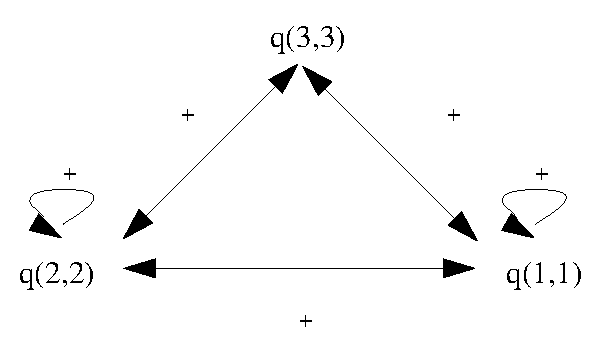
\includegraphics[width=.4\textwidth]{sdg-q-2}
%%\mbox{
%%{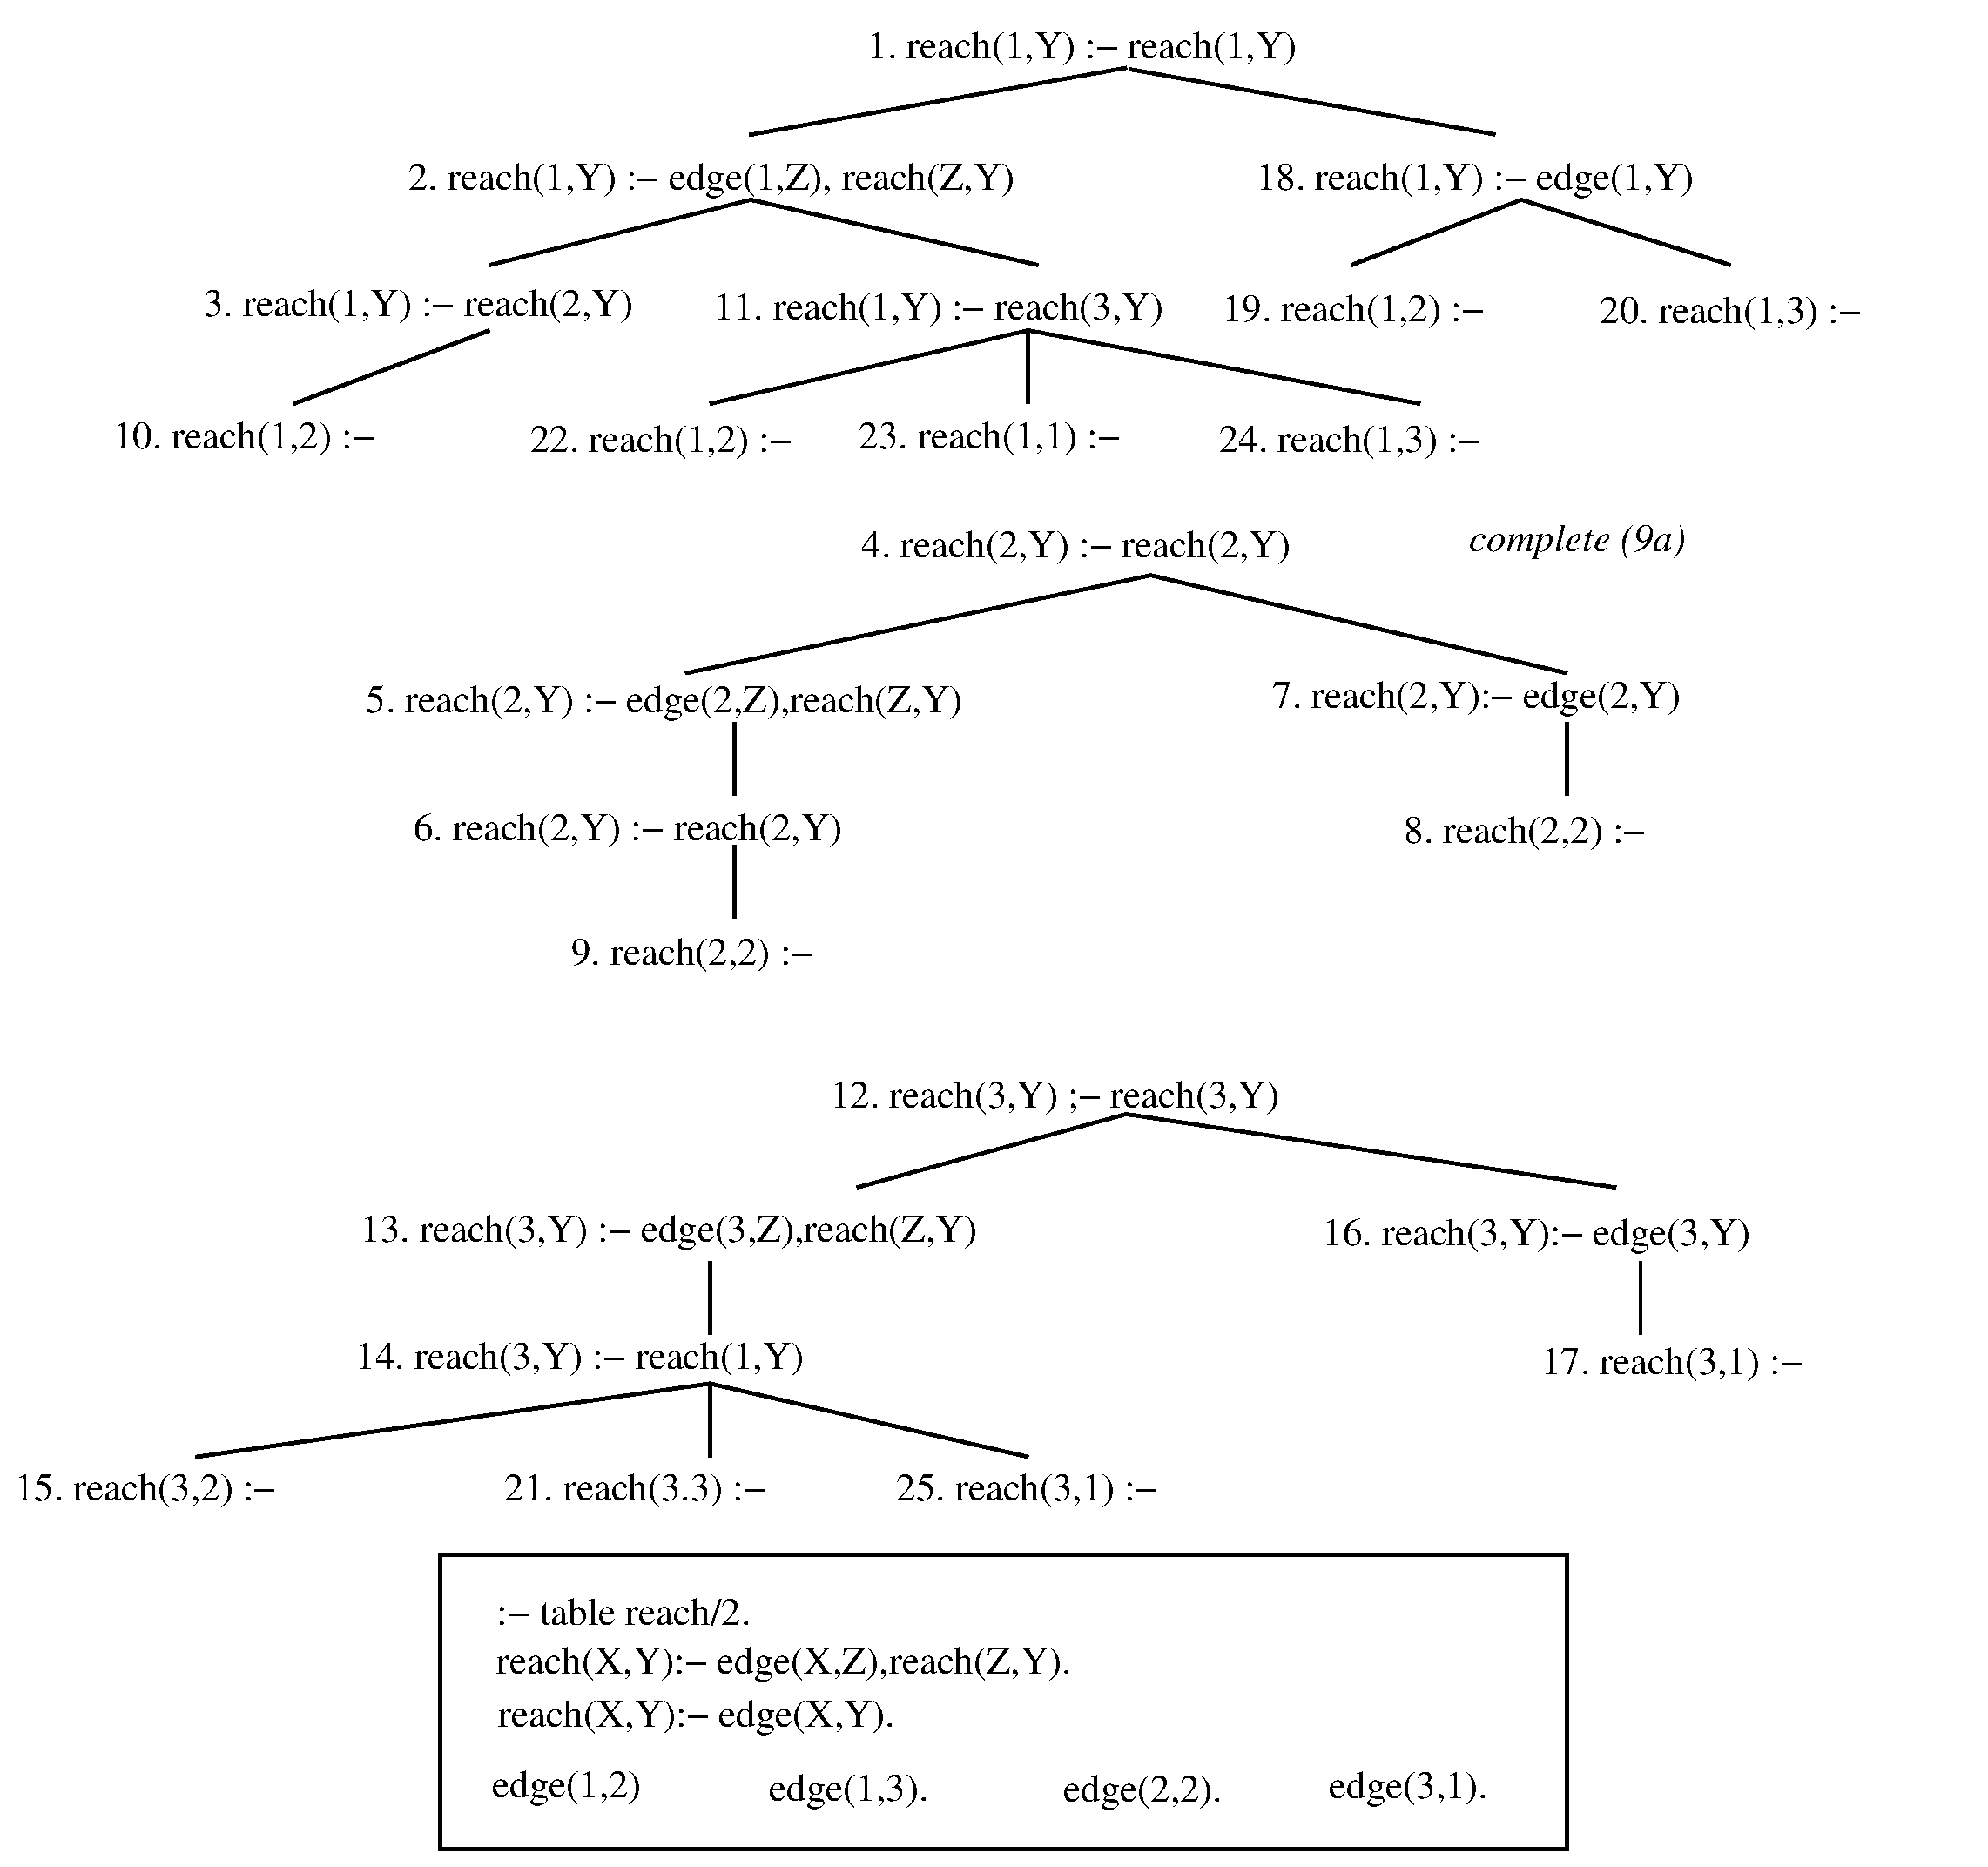
\epsfig{file=slg-forest-local,width=.99\textwidth}}}
\caption{{\em SDG for {\tt ?- q(3,3)} when the derivation is suspended by
  {\tt break/0}}c} \label{fig:sdg-break-1}
\end{figure}
%
This SDG can be produced as follows:
\begin{small}
\begin{verbatim}
| ?- q(3,3).
[ Break (level 1) ]

1: ?- get_sdg_info(F).

F = [subgoal(q(2,3),1,140253373671912,3,0,
             [140253373671672,140253373671792,140253373671912],[]),
     subgoal(q(1,3),1,140253373671792,3,0,
             [140253373671792,140253373671672,140253373671912],[]),
     subgoal(q(3,3),1,140253373671672,3,0,
             [140253373671912,140253373671792],[])]
\end{verbatim}
\end{small}

\end{example}

\ourmoditem{get\_sdg\_subgoal\_info(-SDG)}{get\_sdg\_subgoal\_info/1}{tables}
%
Note that the size of the SDG, which includes dependency edges, may be
quadratic in the number of incomplete subgoals.  When only summary
information about the subgoals in the subgoal dependency graph {\tt
  get\_sdg\_subgoal\_info/1} can be used, rather than {\tt
  get\_sdg\_info/1}.  As with the previous predicate, a list of terms of the form, 
%

{\small
\noindent
{\tt subgoal(Vertex,SCCKey,\_SubgoalKey,CallsTo,Answers,\_PosEdges,\_NegEdges)} }
%

\noindent
is returned, but {\tt \_SubgoalKey} is set to the atom {\tt null}, and
{\tt \_PosEdges} and {\tt \_NegEdges} are both set to the empty list.

This predicate has no error conditions.

\end{description}

\subsubsection{Predicates to Access the Incremental Dependency Graph} \label{sec:idg-preds}

The Incremental Dependency Graph (IDG) is used by XSB's incremental
tabling subsystem to ensure that tables that depend on dynamic facts
or rules are properly updated when the underlying dynamic code
changes.

The Incremental Dependency Graph (IDG) has as vertices those subgoals
whose predicate symbols are incrementally tabled, along with calls to
dynamic predicates that are declared as incremental.  A {\em depends}
edge exists from $S_1$ to $S_2$ iff a call is made to $S_2$ while
computing answers for $S_1$, and if there are no intervening tabled
subgoals between $S_1$ and $S_2$.  An {\em affects} edge is the
inverse of a depends edge.  Edges in the IDG are unsigned.  XSB
maintains both completed and incomplete subgoals in the IDG. (As long
as the tables for these subgoals are not abolished.)

The main predicates for inspecting the IDG as a dependency graph are,
desribed below.  Additionally, Section~\ref{sec:incr-preds1} contains
predicates for examining dependencies among individual subgoals, as
well as returning information about whether a subgoal in the IDG needs
to be updated or not.

\begin{description}
\ourrepeatmoditem{get\_idg\_info(+SubgoalList,-SDG)}{get\_idg\_info/2}{tables}
\ourmoditem{get\_idg\_info(-SDG)}{get\_idg\_info/1}{tables}
%

{\bf {\em Warning: this predicate is not yet implemented}}

Returns information about the {\em Incremental Dependency Graph} (IDG)
as an adjacency list whose form is described in Section~\ref{sec:adjacency-lists}.
%
If there is an empty IDG in the current state, an empty list
is returned.

Recall from the previous section that if the SDG is accessed,
information is returned about all completed subgoals.  The IDG however
may be both very large and disconnected.  Accordingly, {\tt
  get\_idg\_info/2} allows a list of subgoals to be specified, and
returns information about all of the IDG that is connected to any
subgoal in the list; note that the resulting dependency graph may also
be disconnected.  If {\tt get\_idg\_info/1} is called, information is
returned about the entire dependency graph.

{\bf Error Cases}
\bi
\item {\tt SubgoalList} is a variable
\bi
\item 	{\tt instantiation\_error}
\ei
\item {\tt SubgoalList} is not a list
\bi
\item 	{\tt type\_error}
\ei
\item {\tt SubgoalList} contains a predicate that is not tabled
\bi
\item 	{\tt permission\_error}
\ei
\ei
\end{description}

\subsubsection{Predicates to Access the Residual Dependency Graph} \label{sec:rdg-preds}

As discussed in Section~\ref{sec:non-strat}, answers that are
undefined in the well-founded semantics are stored in XSB along with
their delay lists, forming a residual program.  The residual program
can also be represented as a Residual Dependency Graph (RDG).  Using
the RDG, a user may be able to determine why an answer $A$ to a
subgoal $S$ was unexpectedly undefined either because that answer was
involved in or depended on a loop through negation; or because the
answer depended on some other answer that was undefined because of the
use of bounded rationality (Section~\ref{sec:tabling-termination}) or
because of floundering and the use of {\tt u\_not/1}.

The representation of the RDG is slightly different from that of the
other dependency graphs.  The following example illustrates the
reasons for this.

\begin{example}\label{ex:rdg} \rm 
Consider the program 
% 
{\tt 
\begin{tabbing}
fooo\=fooooooooooooooooooooooooooooooo\=ooooooooooooo\=\kill
 \>  :- table p/2. \\
\>           p(1,2). \\
\>           p(1,3):- tnot(p(2,3)).  \\
\>           p(2,3):- tnot(p(1,3)). \> p(2,3):- r(a).\\
\>           r(a):- tnot(r(b)) \\
\>           r(b):- tnot(r(a)).   
\end{tabbing}
}
%
to which the query {?- p(1,X)} was made, generating the tables:
\begin{center}
\begin{tabular}{||l|l||}   \hline
     {\em Subgoal}                 & {\em Answers} \\ \hline \hline
     p(1,X)                     & p(1,2) \\ 
                                & p(1,3):- tnot(p(2,3))| \\ \hline
     p(1,3)                     & p(1,3):- tnot(p(2,3))| \\ \hline
     p(2,3)                     & p(2,3):- tnot(p(1,3))| \\ \hline
                                & p(2,3):- tnot(r(a))| \\ \hline
     r(a)                       & r(a):- tnot(r(b))| \\ \hline
     r(b)                       & r(b):- tnot(r(a))| \\ \hline
\end{tabular}
\end{center}

The residual dependency graph for this program and query would have a
node for each subgoal/answer combination with an undefined truth
value, and a dependency edge for nodes $S_1/A_1$ and $S_2/A_2$ if
$A_2$ occurs in a literal in the delay list for $S_1/A_1$, and the
original subgoal for $A_2$ was $S_2$ in the subcomputation for $S_1$.
The edge also has a sign indicating whether $A_2$ occurs positively or
negatively in the delay list for $A_1$.  In this example, the residual
dependency graph could be conceptually represented as 
%
\begin{verbatim}
     depends_on(p(1,X)/p(1,3),p(2,3)/p(2,3),-).
     depends_on(p(1,3)/p(1,3),p(2,3)/p(2,3),-).
     depends_on(p(2,3)/p(2,3),p(1,3)/p(1,3),-).
     depends_on(p(2,3)/p(2,3),r(a)/r(a),+).
     depends_on(r(a)/r(a),r(b)/r(b),-).
     depends_on(r(b)/r(b),r(a)/r(a),-).
\end{verbatim}
\end{example}

Thus, vertices of the RDG are subgoal/atom pairs, unlike in the other
dependency graphs where they are simply subgoals.  Summarizing, the
RDG which has as vertices those pairs of subgoals and answer atoms,
such that the truth value of the answer atom for that subgoal is {\em
  undefined} in the state of a suspended computation.  A {\em depends}
edge exists from $V_1$ to $v_2$ iff $V_2$ is a delay literal in a
conditional answer for $V_1$.  An {\em affects} edge is the inverse of
a depends edge.  Edges in the RDG are signed indicating positve or
negative dependence.\footnote{An alternative definition of the RDG has
  tabled subgoals as vertices, where subgoal $S_1$ depends on subgoal
  $S_2$ if some answer for $S_1$ depends on some answer for $S_2$.
  Such a representation can be obtained from {\tt
    get\_rdg\_info/[1,2]} below by applying a morphism, as described
  in Section~\ref{sec:dependency-graph-manipulation}.}
%
  A pair $(S,A)$ and its incident edges are removed from the RDG when
  the truth value of $A$ changes, and of course when $S$ is
  abolished.\footnote{The truth value of an atom for a given subgoal may
    change when a suspended state is further evaluated, so that depending when
  a computation is suspended, it is possible though rare that a given
  atom may have a definite truth value when associated with one
  subgoal, but the truth value may not have been propiaged to another
  subgoal.  Note that the truth value of atoms may also change for
  completed subgoals when the {\sc answer completion} operation is
  lazily performed.}

Information about specific vertices and edges of the RDG can be
obtained through predicates such as {\tt get\_residual/2} and {\tt
  variant\_get\_residual/2}.

\begin{description}
\index{residual program}
\predref{get\_residual/2}
\predref{variant\_get\_residual/2}
\index{Incremental Dependency Graph (IDG)}
\index{residual dependency graph}
\ourrepeatmoditem{get\_rdg\_info(+PairList,-SDG)}{get\_rdg\_info/2}{tables}
\ourmoditem{get\_rdg\_info(-SDG)}{get\_rdg\_info/1}{tables}
%

{\bf {\em Warning: this predicate is not yet implemented}}

Returns information about the {\em Residual Dependency Graph} (RDG) as
an adjacency list whose form is described in Section~\ref{sec:adjacency-lists}.
%
If there is an empty RDG in the current state, an empty list
is returned.

Recall from the previous section that if the SDG is accessed,
information is returned about all completed subgoals.  The RDG however
may be both very large and disconnected.  Accordingly, {\tt
  get\_rdg\_info/2} allows a list of subgoal/atom pairs to be
specified, and returns information about all of the RDG that is
connected to any subgoal in the list; note that the resulting
dependency graph may also be disconnected.  If {\tt get\_rdg\_info/1}
is called, information is returned about the entire dependency graph.

{\bf Error Cases}
\bi
\item {\tt PairList} is a variable
\bi
\item 	{\tt instantiation\_error}
\ei
\item {\tt PairList} is not a list
\bi
\item 	{\tt type\_error}
\ei
\item {\tt PairList} contains a predicate that is not tabled
\bi
\item 	{\tt permission\_error}
\ei
\ei

\ourrepeatmoditem{get\_residual\_sccs(+Subgoal,+Answer,-SCCList)}{get\_residual\_sccs/3}{tables}
\ourmoditem{get\_residual\_sccs(+Subgoal,+Answer,-SCCList,-DepList,-SignList)}{get\_residual\_sccs/5}{tables}
%
%At times it can be useful to view the residual program as a directed
%graph, for instance in order to understand why a given answer might be
%undefined.  In a manner somewhat analogous to the incremental
%dependency graph (Section ~\ref{sec:incremental_tabling}) the {\em
%  residual dependency graph} is a directed graph whose nodes are
%subgoal/atom pairs and whose edges are labelled with: 1) a sign
%indicating whether the edge is positive or negative; and 2) the label
%{\em depends on} or {\em affects}.

\index{termination!radial restraint} 
\predref{u\_not/1}
%
{\bf {\em Warning: these predicates may be obsolescent.}}

The residual dependency graph can be constructed in a straightforward
way from {\tt variant\_get\_residual/2}.  However {\tt
  get\_residual\_sccs/[3,5]} provides an alternate view that is
higher-level and much faster.  Given a subgoal/answer pair as
input, each of these predicates constructs SCC-based information about
the residual dependency graph via structures of the form:
%
\begin{center}
{\tt ret(Subgoal,Answer,SCCKey)}.
\end{center}
%
where {\tt SCCKey} is a generated key for the SCC to which the
Subgoal/Answer pair belongs. Two subgoal/answer pairs are in the same
SCC iff they have the same {\tt SCCKey}; however no other dependency
information can be otherwise directly inferred from the
index~\footnote{The actual number used for each SCC key depends on how
  RDG happens to be traversed; as a result it is best to rely on the
  key only as a ``generated'' name for each SCC.}.

To obtain dependency information, {\tt get\_residual\_sccs/5} also
returns a list indicating the direct dependencies among the SCCs,
along with a list indicating whether each SCC contains a negative
edge.  For Example~\ref{ex:rdg}, the SCC information would have a form
such as:
\begin{verbatim}
[ ret(p(1,X),p(1,3),1), ret(p(1,3),p(1,3),2), ret(p(2,3),p(2,3),2),
  ret(r(a),r(a),3), ret(r(b),r(b),3) ]
\end{verbatim}
%
The dependency list would have a form such as:
\begin{verbatim}
[ depends(1,2), depends(2,3) ]
\end{verbatim}
while the sign list would have a form such as:
\begin{verbatim}
[ sign(1,no_neg), sign(2,neg), sign(3,neg) ]
\end{verbatim}
If it is necessary to know which subgoal(s) in {\tt SCC1} directly
depends on which subgoal(s) in {\tt SCC2}, the information can be
easily reconstructed from the output of {\tt
  get\_residual\_sccs/[4,5]} using {\tt variant\_get\_residual/2}.  A
similar approach can be used to determine the actual edges within a
given SCC.

SCC detection is implemented using Tarjan's algorithm~\cite{Tarj72} in
C working directly on XSB's data structures.  The algorithm is
$\cO(|V| + |E|)$ where $|V|$ is the number of vertices and $|E|$ the
number of edges in the dependency graph.  As a result, {\tt
  get\_residual\_sccs/3} provides an efficient means to materialize
the high-level topography of the dependency graph~\footnote{Currently,
  the materialization of dependency information between SCCs is
  implemented in a naive manner, so that {\tt get\_residual\_sccs/6}
  is $\cO(|V|^2)$.}.

%These predicates implement Tarjan's algorithm~\cite{Tarj72} in C
%working directly on XSB's data structures.  The algorithm is $\cO(|V|
%+ |E|)$ where $|V|$ is the number of vertices and $|E|$ the number of
%edges in the dependency graph.  As a result, these predicates provide
%an efficient means to materialize the dependency graph, even if SCC
%information per se is not required
  
\index{radial restraint}
\index{termination!radial restraint}
\predref{u\_not/1}
\predref{get\_residual\_sccs/5}
\ourrepeatmoditem{explain\_u\_val(+Subgoal,+Answer,-Reason)}{explain\_u\_val/3}{tables}	
\ourmoditem{explain\_u\_val(+Subgoal,+Answer,-Sccs,-Deps,-Signs,-Reason)}{explain\_u\_val/6}{tables}	
%
The XSB predicate
%
{\tt explain\_u\_val(+Subgoal,+Answer,?Reason)}
\noindent
can be used to query why {\tt Answer} is undefined when derived in an
evaluation of {\tt Subgoal}.  {\tt Reason} may be
\begin{itemize}
\item {\tt negative\_loops(cycle)} if the derivation of {\tt Answer} involves a
  loop through though negation that includes {\tt Answer} itself.
%
\item {\tt negative\_loops(dependent)} if the derivation of {\tt
  Answer} depends on an atom that is involved in a loop through though
  negation.
%
\item {\tt unsafe\_negation} if the derivation of {\tt Answer} depends
  on a negative subgoal that is non-ground (XSB does not automatically
  perform subgoal reordering).  The action of making a non-ground
  subgoal undefined is performed by {\tt u\_not/1}.
%
\item {\tt bounded\_rationality} if the derivation of answer depends
  on bounded rationality based on radial restraint~\cite{GroS13}.
\end{itemize}
%
These reasons are not exclusive, and complex derivations may well
involve several of the above reasons.

{\tt explain\_u\_val/[3,6]} is based on the structures returned by
{\tt get\_residual\_sccs/[3,5]}.  While {\tt
  get\_residual\_sccs/[3,5]} is reasonably fast, it can take a
peceptable time to analyze large residual programs containing many
thousands of SCCs.  Accordingly, {\tt explain\_u\_val/6} can reuse
dependency structures returned by {\tt get\_residual\_sccs/[3,5]},
which can be useful for justification systems and other applciations.

\begin{example} \rm
After executing the query {\tt p} to the program
%
\begin{verbatim}
:- table p/0, q/0, r/0, s/1.
p:- q,tnot p.                 p:- s(f(f(f(f(0))))).

q:- tnot r.                   r:- tnot q.

s(f(X)):- s(X).               s(0).
\end{verbatim}
%
where the bounded rationality size has been set to 3.  The query {\tt
  explain\_u\_val(p,P,Reason)} will bind {\tt Reason} to {\tt
  negative\_loops(cycle)}, to {\tt negative\_loops(dependent)}, and
to {\tt bounded\_rationality} (this ordering is not guaranteed).
\end{example}
\end{description}

\subsubsection{Filtering, Manipulating, and Summarizing Dependency Graphs} \label{sec:dependency-graph-manipulation}

\begin{description}
\ourmoditem{morph\_dep\_graph(+DG\_In,+Morph,-DG\_Out)}{morph\_dep\_graph/3}{tables}
%
This predicate takes as input {\tt DG\_In}, a dependency graph in
adjacency list format and returns its image, {\tt DG\_Out}, under the
graph homomorphism {\tt Morph}.  {\tt Morph} is a predicate symbol
that identifies a 2-ary predicate, {\tt Morph(+In,-Out)} that is
functional on {\tt In} and that maps the Herbrand Base of the current
program into itself.  The syntax of {\tt DG\_In} and {\tt DG\_Out} is
described at the beginning of Section~\ref{sec:adjacency-lists}.

To recall the definition of a graph homomorphism (cf. e.g.,
~\cite{Hara69}) a functional notation is used for {\tt Morph/2}.  {\tt
  DG\_Out} is a graph such that the vertices of {\tt DG\_Out},
$vertices({\tt DG\_Out})$ is the set:
\[
\{ morph(V) | V \in vertices({\tt DG\_In}) \}
\]
while the edges of {\tt DG\_Out}, $edges({\tt DG\_Out})$ are the sets
\[
\{ \langle morph(V_1),morph(V_2) \rangle | \langle V_1,V_2 \rangle \in edges({\tt DG\_In}) \}
\]
We adapt this definition to signed dependency graphs by mapping all
positive adjacenct edges into a positive set, and negative adjacent
edges into a negative set.

The power of {\tt morph\_dep\_graph/3} arises when the numbers of
vertices and edges of {\tt DG\_In} is large, and {\tt morph/2} ensures
that numbers for {\tt DG\_Out} are much smaller -- thus allowing
recognizable patterns to emerge.

For efficiency reasons, a special condition, ${\cal C}_1$, is assumed
  about {\tt morph/2}: that if two elements of its range unify, then
  they must be identical.  For instance, a morphism $M_1$ that reduced
  the maximum depth of each non-variable argument of a term by 1 would
  not fit this condition, since $M_1(f(a,g(h(b)))) = f(X_1,g(h(X_2)))$
  while $M_1(f(a,g(b))) = f(X_1,g(X_2))$, which unify.  On the other
  hand, a morphism that abstracts each argument to have a maximal
  fixed depth would fulfill the condition.  In any case, as long as
  ${\cal C}_1$ is observed, {\tt morph/2} may instantiated by an
  abstraction function as used elsewhere in this manual: i.e., a
  function such that $morph(Term)$ subsumes $Term$.  However, other
  morphisms may also be useful as demonstrated in
  Example~\ref{ex:morph-sdg} below.

While the syntax of {\tt SDG\_Out} is the same as that of {\tt SDG\_In},
the meaning of the arguments differs slightly.  {\tt SDG\_Out} is a
list of terms of the form:

{\tt subgoal(MorphSubg,null,Key,CallsTo,Answers,PosKeyList,NegKeyList)} 

such that 

\bi
\item {\tt MorphVert} is $morph({\tt Vertex})$ for one or more
  subgoals that are vertices of {\tt DG\_In}
\item The second argument, which represents SCC information in the
  original dependency graph, is the atom {\tt null} when a morphism is
  applied, since SCC information is not preserved in general.
\item {\tt Key} is an atom identifying {\tt MorphVert}.  Note that
  while each subgoal in {\tt DG\_In} corresponds to e.g., a tabled
  subgoal, a given subgoal image in {\tt DG\_Out} may not correspond to
  a tabled subgoal in the current state.  Thus a table entry handle
  may not be available, so generated keys are used in {\tt DG\_Out}.
\item {\tt CallsTo} If {\tt DG\_In} originated from an SDG or IDG, {\tt
  CallsTo} is the sum of the number of calls to every subgoal $S \in$
  {\tt DG\_In} such that $morph(S) = {\tt MorphVert}$.  Otherwise, {\tt
    CallsTo} is 0.
\item {\tt Answers} If {\tt DG\_In} originated from an SDG or IDG, {\tt
  Answers} is the sum of the number of answers for every subgoal $S
  \in$ {\tt DG\_In} such that $morph(S) = {\tt MorphVert}$.  Otherwise,
     {\tt Answers} is 0.
\item {\tt PosKeyList} is a list of the keys to those vertices adjacent
  to {\tt MorphSubg} with positive sign as described above.
\item {\tt NegKeyList} is a list of the keys to those vertices adjacent
  to {\tt MorphSubg} with negative sign as described above.
\ei

\begin{example} \rm \label{ex:morph-sdg}
Continuing Example~\ref{ex:get-sdg}, let {\tt mymorph} identify the
predicate

\begin{verbatim}
mymorph(Term,NewTerm):-
        Term =.. [F,A1,A2],
        map_arg_1(A1,NewA1),
        NewTerm =.. [F,NewA1,A2].

map_arg_1(2,1):- !.
map_arg_1(X,X).
\end{verbatim}
Thus {\tt mymorph/2} maps {\tt q(2,1)} to {\tt q(1,1)} and maps
both {\tt q(1,1)} and {\tt q(3,1)} to themselves.  Then if {\tt DG\_In}
is instantiated to the SDG produced in Example~\ref{ex:get-sdg}, the
goal {\tt ?- morph\_dep\_graph(DG\_In,mymorph,DG\_Out)} would produce:

\begin{verbatim}
SDG\_Out = [subgoal(morph80,q(1,3),6,0,[morph80,morph81],[]),
          subgoal(morph81,q(3,3),3,0,[morph80],[])
\end{verbatim}
\end{example}

{\bf Error Cases} 
\bi
\item 	{\tt Morph} is not an atom
\bi
\item 	{\tt type\_error}
\ei
%
\item 	{\tt DG\_Out} is not a variable
\bi
\item 	{\tt type\_error}
\ei
%
\item 	{\tt DG\_In} is not an adjacency list as described above
\bi
\item 	{\tt misc\_error}
\ei
\ei
%
\ourmoditem{dep\_graph\_scc\_info(+SDG,-ListOut)}{dep\_graph\_scc\_info/2}{tables}
%
Given an SDG representation in the adjacency list format described
above, this predicate returns information about the SCCs that are
currently under evaluation.  Upon success {\tt ListOut} will contain a
term

{\tt scc(SCCIndex,NumSubgoals,NumAnswers,NumPosEdges,NumNegEdges)}

for each SCC under evaluation, such that:

\bi
\item {\tt SCCIndex} is the index of the SCC
\item {\tt NumSubgoals} is the number of subgoals in the SCC
\item {\tt NumAnswers} is the total number of answers for all subgoals in the SCC
\item {\tt NumPosEdges} is the total number of positive edges within the SCC.
\item {\tt NumNegEdges} is the total number of negative edges within the SCC.
  \ei

\ourmoditem{print\_sdg\_info}{print\_sdg\_info/0}{tables}
%
Prints the current SDG to {\tt stdout} in a readable
manner.\footnote{This predicate, along with {\tt
    print\_sdg\_subgoal\_info/0} replaces the predicate {\tt
    print\_incomplete\_tables/0}, which was included in previous
  releases.}

\ourmoditem{print\_sdg\_subgoal\_info}{print\_sdg\_subgoal\_info/0}{tables}
%
Prints summary subgoal information about the current SDG to {\tt stdout} in a
readable manner.

\ourmoditem{print\_dep\_graph(+DG)}{print\_dep\_graph/1}{tables}
%
Prints a dependency graph {\tt DG} (whether its an SDG, IDG, or RDG)
to {\tt stdout} in a simple, but readable manner.
%
\begin{example}
Continuing from Example~\ref{ex:morph-sdg}, if 

\begin{verbatim}
SDG = [subgoal(morph80,q(1,3),6,0,[morph80,morph81],[]),
          subgoal(morph81,q(3,3),3,0,[morph80],[])
\end{verbatim}

then {\tt print\_dep\_graph(SDG)} would output

\begin{verbatim}
Subgoal: q(1,3)
        Number of calls to this subgoal 6; Number of answers 0
        Affects positively q(1,3) ; q(3,3)
Subgoal: q(3,3)
        Number of calls to this subgoal 3; Number of answers 0
        Affects positively q(1,3) 
\end{verbatim}
\end{example}

\end{description}

\subsection{Summary: Inspection Predicates}

XSB provides a number of ways to inspect a tabled derivation,
including directly through the tables, or through one of the
dependency graphs: the IDG, RDG or SDG.  Specifically, some useful
inspection predicates available in XSB are:

\begin{itemize} 
\item {\tt statistics/[0,1,2]} (Section~\ref{environmental}) is a
  highly useful general-purpose predicate that provides an important
  summary of how memory is used by the XSB process or thread, the
  amount of time used by the process or thread, along with various
  counts of tabling operations and measures of table space.

\item {\tt table\_dump/[2,3]} (Section~\ref{sec:table-dump}) allows
  directed and iterative inspection of the current set of tabled
  subgoals and their answers, at various levels of summary
  aggregation.

\index{Incremental Dependency Graph (IDG)} 
\index{residual program}
\index{residual dependency graph}
\item Inspection of the Incremental Dependency Graph can be made via
  the predicate {\tt get\_idg\_info/[1,2]}
\footnote{These predicates
    are not yet implemented: although {\tt tt get\_incr\_sccs/[1,2]},
    and {\tt get\_incr\_sccs\_with\_deps/[2,3]} have been.} together
  with predicates for dependency graph manipulation such as {\tt
    morph\_dep\_graph/3} and {\tt dep\_graph\_scc\_info/3}
  (cf. Section~\ref{sec:dependency-graph-manipulation}).
%
 More targeted inspection of specific edges and dependencies of the
 Incremental Dependency Graph is supported through {\tt
   incr\_directly\_depends/2} and {\tt incr\_trans\_depends/2}
 (cf. Section~\ref{sec:incr-preds1}).

\item Inspection of the Subgoal Dependency Graph can be obtained
  through the predicate {\tt get\_sdg\_info/1}, and its information
  analyzed through predicates for dependency graph manipulation such
  as {\tt morph\_dep\_graph/3}, and {\tt dep\_graph\_scc\_info/2}
  (cf. Section~\ref{sec:dependency-graph-manipulation}).  Note that
  {\tt get\_sdg\_info/1} returns information concerning incomplete 
  subgoals {\em only}.

\item Inspection of the Residual Dependency Graph can be made via the
  predicate {\tt get\_rdg\_info/[1,2]},\footnote{This predicate is not
    yet implemented: although {\tt tt get\_residual\_sccs/[1,2]} has
    been.} together with dependency graph manipulation predicates such
  as {\tt morph\_dep\_graph/3} and {\tt dep\_graph\_scc\_info/3}.
  (cf. Section~\ref{sec:dependency-graph-manipulation}).  The
  predicates {\tt get\_residual/2} and {\tt variant\_get\_residual/2}
  allow the residual program to be viewed as sets of clauses.
  Finally, {\tt explain\_u\_val/3} can be used to indicate why a given
  atom has the truth value {\em undefined} rather than {\em true} or
  {\em false} (cf. Section~\ref{sec:table-inspection}).
\end{itemize}

All of these predicates, except for {\tt get\_sdg\_info/1}, can be
used to retrospecitively analyze any completed derivation, as long as
the derivations tables have not been abolished.  In addition, all of
the predicates can be used to analyze an onoging derivation by
suspending the derivation and then examining the computation from a
subsidiary command-line interpreter.  This can be especially important
for long-running computaiotions or those that take a lot of space.

In XSB, a computation can be suspended in several ways, depending a
user's tastes in and needs for debugging:

\bi 
\item By a call to {\tt break/0}.  This is usually best done by
  calling {\tt break/0} as part of a handler for {\tt timed\_call/2},
  but {\tt break/0} can also be called explicitly from a program.
%
\item By hitting ctrl-C if XSB is running in stand-alone mode

\item By setting a {\em tripwire} as introduced below
  (Section~\ref{sec:tripwire}).  
%
\ei

\index{tripwires}
\subsection{Setting Tripwires on Tabled Derivations} \label{sec:tripwire}
%
A tripwire represents an unexpected property of a derivation: such as
an excessive use of time or memory; an unexpected number or complexity
of tabled subgoals or answers; or an unexpected number of mutually
dependent tabled subgoals.  Depending both on the class of a tripwire
and on how XSB's flags are set, a tripwire may have different effects.
Any tripwire may be treated as an error so that it throws an exception
just as any other error.  {\em Inspectable} tripwires may additionally
be considered as inspection points, and when hit may suspend the
derivation and create a break point.\footnote{Note that such a
  suspension makes available for inspection the state of the
  derivation at the point the tripwire was activated.  If inspection
  points were implemented using ISO errors, state could only be made
  available at the point where the error was {\em caught}, whose state
  may differ greatly from the point where the error occurred (i.e.,
  where the tripwire was hit).}
%
In such a case, a short explanation will be made of how a tripwire was
encountered, along with suggestions about how to further inspect the
suspended derivation.\footnote{
  %% 
  This is the default behavior for XSB:
  handling of tripwires can be overridden by the user,
  as explained later in this section.
}
%%
{\em Correctable} tripwires are a subset of
inspectable tripwires for which an automatic action may be taken to
remedy the situation, such as rewriting a subgoal or an answer whose
size is greater than a given limit, by using subgoal abstraction or
answer restraint.

Tripwires may be set in various ways: most can be set and viewed at a
session level using Prolog flags, others can also be set at the
predicate level via the {\tt table/1} declaration, while still others
can only be set by explicit programming.  Tripwires thus represent a
coordinated set of tools for understanding bounds on a tabled
derivation, rather than a unified API.

For a tripwire {\tt T} that can be set and viewed as a Prolog flag,
the flag name has the form {\tt tripwire(T)}, and this flag has two or
more values.  An {\em action}, designated {\tt action(A)}, indicating
the action to take such as {\tt error}, {\tt suspend}, or other
actions; and one or more parameters, designated {\tt limit(P)}.
For example, if a user wants to be able to suspend and inspect a
computation whenever it has an active recursive component (SCC) with
over 100 subgoals, she can execute the following directives:

{\tt ?- set\_prolog\_flag(tripwire(max\_scc\_subgoals),limit(100)).}

{\tt ?- set\_prolog\_flag(tripwire(max\_scc\_subgoals),action(suspend)).}

We discuss various types of tripwires in turn, and provide informal
guidelines for inspecting a derivation when a given tripwire has been
hit.

\subsubsection{Tripwires Based on Resource Limits}
%
Hitting a resource tripwire reflects the fact that a derivation is
taking more time or using more memory than expected.  A resource
tripwire is a user-imposed limit, rather than an external limit
imposed by the platform or operating system, and thus differs from an
ISO resource error.

\index{tripwires!timed call} 
\predref{timed\_call/2}
\predref{timed\_call\_modify/1}
%
Time-based resource tripwires can easily
be programmed using a handler to {\tt timed\_call/2}.  Time-based
tripwires are inspectable, so such a handler might throw an error
after a derivation has taken a certain amount of CPU time, or call
{\tt break/0} to implement periodic inspection points, or implement
other periodic analytics or monitoring.  The parameters for timed call
can be changed whenever the timed call is suspended by {\tt
  timed\_call\_modify/1}.  See Section~\ref{sec:timed-call} for more
details.

\index{tripwires!max\_memory} An inspectable memory-based resource
tripwire can be set via the Prolog flag {\tt tripwire(max\_memory)},
so that the tripwire will be hit whenever XSB uses more than a given
total amount of memory.  This amount can be set either as an integer,
representing an absolute number of kilobytes or as a floating point
number indicating a percentate of the RAM of the platform upon which
XSB is executing.  Currently, a memory-based tripwire can only throw
an error.

\paragraph{Guidelines for Analysis of Resource-based Tripwires}  \ \\

{\bf {\em Note that the numbers and sizes below are for example
    purposes only.  If memory limits are set to, say, a gigabyte or
    more of memory, and time limits are set to several seconds, the
    numbers and sizes may be several orders of magnitude more than
    those shown below.}}

If a resource tripwire is hit, the best course of analysis usually
starts with viewing the output of {\tt statistics/[0,1]}.  
\bi
\item {\em Check that there are a large number of incomplete tables}
  This can be determined, for instance, using the output of {\tt
    statistics/0}, by a line near the end of the memory
  table.~\footnote{This line is not printed out if there are no
    incomplete tables.}  E.g.:
%
{\small \begin{verbatim}
        (501227 incomplete table(s) in 89 SCCs)
\end{verbatim} }

\bi
\item If there are a large number of incomplete tables, XSB's stask
 space is likely to be high also, since an incomplete table $T$ needs
 to maintain many details of its derivation state to ensure all
 answers for $T$ are returned to all calls to $T$.  In this case, the
 predicates for analyzing the Subgoal Dependency Graph of the
 suspended derivation can be used (Section~\ref{sec:sdg-preds}).  {\em
 Note that, here and below, when there are a large number of
 incomplete tables, information returned by {\tt get\_sdg\_info/1}, as
 well as by {\tt get\_idg\_info/1} and {\tt get\_rdg\_info/1} may need
 to be filtered or manipulated using the predicates in
 Section~\ref{sec:dependency-graph-manipulation}.}
\ei

\item {\em Otherwise, Check whether there are a large number of
 completed subgoals.} If there are not many incomplete
 tables but the table space seems large, {\tt statistics/[0,1,2]}
 indicates both the total number of tabled subgoals and the total
 number of answers.  In this case.  For instance, the beginning of the
 summary of tabling operations might contain information such as:

%
{\small 
\begin{verbatim}
 Tabling Operations
  12 subsumptive call check/insert ops: 9 producers, 3 variants,
  0 properly subsumed (0 table entries), 0 used completed table.
  0 relevant answer ident ops.  0 consumptions via answer list.
  1065417 variant call check/insert ops: 938125 producers, 127292 variants.
  46210 answer check/insert ops: 46210 unique inserts, 0 redundant.
\end{verbatim} } 

This indicates that there are 1,065,417 subgoals (complete or
 incomplete) tabled with call variance, and 12 subgoals tabled with
 call subsumption.  Among all subgoals there are 46,210 ansewrs.  
%
\bi
\item To understand details of overall table space usage, {\tt
  table\_dump/[2,3]} can be called to provide further information
  (Section~\ref{sec:table-dump}).  
\ei
%
\item {\em Check whether the IDG is large.}  In addition to simply
  having a large number of subgoals (incomplete or complete) and
  answers, the use of incremental dependency, which maintains an IDG,
  has an effect on memory.  {\tt statistics/[0,1]} indicates when
  incremental tabling is being used heavily, by a line towards the
  bottom of the output, such as:
%Total number of incremental subgoals created: 50
{\small \begin{verbatim}
Currently 501688 incremental subgoals, 781432 dependency edges
\end{verbatim} }
%
\bi
\item When there are large numbers of incrementally tabled subgoals
  and dependency edges, {\tt get\_idg\_info/1}
  (Section~\ref{sec:idg-preds}) can be used to obtain a global view of
  the IDG.  Note that incremental tabling does require more memory for
  completed tables than non-incremental tabling, due to the need to
  retain the IDG so that tables can be updated when dynamic code
  changes.
%
\ei
\item {\em Check whether there are a large number of answers whose
  truth value is {\em undefined}}.  This is indicated, for instance,
  by lines at the end of the summary of tabling operations in {\tt
    statistics/0}.~\footnote{These lines are not printed out if there are no
    incomplete tables.}  E.g.:
{\small \begin{verbatim}
   80005 DEs in the tables (space: 3932480 bytes allocated, 3840560 in use)
   40005 DLs in the tables (space: 983200 bytes allocated, 960280 in use)
\end{verbatim} }
%
\bi
If there is indication that there are a large number of answers with
 truth value {\em undefined}{\tt get\_rdg\_info/[1]} and/or {\tt
 explain\_u\_val/2} can be used to understand the dependencies among
 these answers.  
\ei
\ei

\subsubsection{Tripwires Based on Properties of a Tabled Derivation}
%
Theoretically speaking, in a pure logic program if a tabled derivation
 is not terminating it is because there are an unbounded number of SLG
 trees, or because one or more of the SLG trees is of unbounded size.
  The former case indicates that a computation has an unbounded number
 of subgoals, while the latter indicates that one or more subgoals has
 an unbounded number of answers.  In a similar manner, terminating but
 expensive derivations also may have too many subgoals, too many
 answers, or too many dependencies among incomplete subgoals.  We
 consider these cases in turn.

\bi
\item {\em There are too many tabled subgoals} 
\bi
\item {\em There are a potentially unbounded number of tabled subgoals
 in a pure program.}\/ In this case, there must be a potentially
 unbounded number of {\em distinct} tabled subgoals in the derivation.
  If this happens using ca`v`vll variance, this situation can
 sometimes be addressed by using call subsumption instead.  However
 termination can {\em always} be ensured by using subgoal abstraction,
 as long as a derivation produces only a finite number of answers
 (cf. Section~\ref{sec:tabling-termination} and \cite{RigS14}).  XSB
 allows subgoal abstraction to be applied based on term size either
 globally through the tripwire {\tt max\_table\_subgoal\_size}, or on
 a predicate-by-predicate basis through tabling directives.  In other
 words, when a tabled subgoal, $S_{big}$, is called whose size is
 greater then the limit specified for its predicate, a tripwire is
 activated, and various actions can be specified.  In many -- perhaps
 most -- cases, the best action is simply to abstract $S_{big}$.
  However it is also possible to suspend and inspect the derivation so
 that the causes that led to $S_{big}$ can be analyzed.  As a final
 alternative, an error can be thrown, which is the default action.

\item {\em There are a potentially infinite number of subgoals in a
 program with arithmetic.}.  Due to the manner in which numbers are
 represented in XSB, XSB's size metric would permit a potentially
 infinite number of subgoals if numbers occurred within these
 subgoals.  The tripwire {\tt max\_incomplete\_subgoals} allows a
 limit to be set on the maximal number of incomplete subgoals.  If a
 derivation exceeds that limit, the computation may be suspended, or
 an error thrown.

\item {\em There are a finite but large number of tabled subgoals.}\/
 A separate problem from those above can happen as follows.  If a
 program is written over a language that has a finite but large number
 of constant symbols, then a program that generates subgoals of the
 form
\[
   p(c_i,c_j,c_k,X)
\]
  will theoretically terminate, but may be too inefficient for
 practical purposes.  This problem can be addressed by the tripwrite
 {\tt max\_incomplete\_subgoals} just discussed, but it is often
 helpful to have a different size limit for cases where there are a
 large number of subgoals within the {\em same} SCC.

 The tripwire {\tt max\_scc\_subgoals} allows such a limit to be set
 on the maximal number of incomplete subgoals in any recursive
 component.  If a derivation exceeds that limit, the computation may
 be suspended, or an error thrown.  This situation is similar to that
 of simply having too many incomplete subgoals, but may suggest a
 different focus when analyzing a suspended computation.  In addition,
 the number of dependencies can rise quadratically with the absolute
 size of an SCC.  As a result, it often makes sense to have different
 limit for the size of a single (incomplete) SCC and for the number of
 incomplete subgoals overall.
%

{\em Guidelines for Analysis} If the computation is producing too many
 tabled subgoals the suspension may have been triggered by one of the
 tripwires: {\tt max\_table\_subgoal\_size}, {\tt
 max\_incomplete\_subgoals} or {\tt max\_scc\_size}.  In any of these
 cases, the suspension or error message will indicate the tripwire
 that has been hit.  The number of incomplete subgoals can be seen
 from the output of {\tt statistics/0}.  The inspection predicates of
 Section~\ref{sec:dep-graph} can be used to examine these subgoals and
 their dependencies.
%
\ei
\ei 

\bi

\item {\em There are too many tabled answers.} The approaches to this
  situation are similar in spirit to the cases of too many subgoals.
%
\bi
\item {\em One or more subgoals has an unbounded number of answers.}
  In this case, termination can be ensured by using radial restraint,
 which abstracts answers in a manner that is sound with respect to the
 well-founded semantics and can ensure that a derivation will produce
 only a finite number of answers
 (cf. Section~\ref{sec:tabling-termination} and\cite{GroS13}), XSB
 allows radial restraint to be applied based on term size in two ways.
  First, restraint can be applied globally through the tripwire {\tt
 max\_table\_answer\_size}.  Second, XSB allows restraint to be
 declared at a predicate-by-predicate basis.  In other words, when an
 answer, $A_{big}$, is to be added to a table, and its size is greater
 then the limit specified for its predicate, a tripwire is activated,
 and various actions can be specified.  In many cases, the best action
 is simply to abstract $A_{big}$, which gives it the truth value {\em
 undefined} for that answer. However it is also possible for the
 derivation to be suspended so that the causes that led to $A_{big}$
 can be analyzed.  As a final alternative an error can be thrown; this
 is the default action for XSB.

\item {\em There are a finite but large number of tabled answers.}\ As
  with subgoals, checking for the depth of an answer may not catch
  certain causes of inefficency. If a program is written over a
  language that has a large number of constant symbols, then a program
  that generates answers of the form
\[
   p(c_i,c_j,c_k,c_l)
\]
  will theoretically terminate, but may be too inefficient for
  practical purposes.  

  To address such situations, XSB has the tripwire {\tt
    max\_answers\_for\_subgoal} which is hit if any subgoal has more
  than the specified number of answers.  If a derivation exceeds that
  limit, the computation may be suspended, or an error thrown.
%
 \ei {\em Guidelines for Analysis} If the computation is producing too
 many tabled answers, a suspension may be triggered by one of the
 tripwires: {\tt max\_table\_answer\_size}, or {\tt
 max\_answers\_for\_subgoal}.  In any of these cases, the suspension
 (or error message) will indicate the subgoal whose number of answers
 hit the tripwire.  The number and shape of answers for that subgoal
 and others can be viewed through the {\tt table\_dump} library
 (Section~\ref{sec:table-dump}).  If some answers are undefined, the
 predicates {\tt get\_rdg\_info/1} and {\tt explain\_u\_val/2} can be
 used to explore dependencies among the answers.  In addition,
 dependency graph analysis based on the predicates {\tt
 get\_sdg\_info/1} and {\tt get\_idg\_info/1} can help locate areas of
 code that caused the profusion of answers.

 \ei

\subsubsection{The Suspend Action for Flag-Based Tripwires}

If the action {\tt suspend} is specified for a given flag-based
 tripwire $T$, (i.e., a tripwire other than one based on {\tt
 timed\_call/2}), then hitting $T$ causes XSB to take a given action.
  By default, this action is to enter a break level from which the
 computation can be inspected. (This default action for {\tt suspend}
 can be overridden.)  A preamble to the break level is also presented
 that describes certian values pertaining to the state of the
 computation, along with an attempt to summarize what the situation
 means.  The preamble for the tripwire {\tt max\_incomplete\_subgoals}
 appears as follows.

%----------------------------------------------------------------------------------------
\begin{small}
\begin{verbatim}
There are currently 11 incomplete tabled subgoals, which exceeds the limit set by the 
flag 'max_incomplete_subgoals'.  These subgoals are in 11 separate recursive components.

The number of incomplete recursive components is close to the number of incomplete 
subgoals, and furthermore, nearly all of these recursive components are trivial.

This information indicates a likelihood that the program is performing some sort of 
structural recursion using tabling (i.e., recursing through a list, performing numeric 
iteration, etc.)

To remedy, check that the recursion is well-founded.  If so, consider executing the 
recursion using a non-tabled predicate, or consider using hash-cons tabling to reduce 
the space required for tables, then increase the value of the flag.

  * To continue, reset the flag and then type Ctrl-d
  * To abort the suspended derivation, enter the command 'abort/0'
  * To inspect the incomplete tabled subgoals, enter the command 'print_sdg_info/0'
\end{verbatim}
\end{small}
%----------------------------------------------------------------------------------------

From within a break level thrown by a tripwire, a user can perform
 most queries and commands with two important exceptions.

\begin{itemize}
\item No tabled goals or subgoals may be executed.  Of course once the
 break is exited, the original comptuation can be continued, and
 tabled subgoals can be executed as usual.
\item Reconsulting a file containing code upon which the original
 query depends may throw an error.
\end{itemize}

There are situations where the action of breaking to allow a user can
 inspect a query isn't suitable -- if XSB is embedded into a process,
 for instance, or is part of some other application.  In such a case,
 the user can override XSB's default behavior by asserting into the
 {\tt user} module a {\em tripwire handler}, which will be executed
 when a given tripwire is hit.  For instance, the tripwire {\tt
 max\_table\_subgoal\_size} would use the tripwire {\tt
 max\_table\_subgoal\_size\_user\_handler/0}.  Subject to the
 constraints above, the handler may perform any actions desired,
 including increasing the tripwire limit, adjusting its action,
 changing runtime tabling properties, or simply writing to a
 log.\footnote{As a further example, when XSB supports the language
 Ergo the tripwire may set on forest logging to support termination
 analysis via the Terminyzer tool.}

A handler that is called when a tripwire is hit has some resemblences
 to a handler called when an error is caught, but there are important
 differences.  A condition triggering a tripwire might or might not
 reflect an error in a program.  So the handler is invoked when the
 tripwire is hit, rather than after exiting portions of that
 derivation as is the case when an error is caught.  If the user wants
 to exit some or all of a derivation when a tripwire is hit, it is
 simple to change the tripwire's action to error, and arrange to catch
 the error with a suitable handler.

\subsubsection{Summary of Flag-Based Tripwires}
%
Each of the tripwires described below can be queried and set via
 prolog flags.  For instance the query

\begin{verbatim}
| ?- current_prolog_flag(tripwire(max_table_subgoal_size),Property).

Property = limit(12)
Property = action(error);
\end{verbatim}
indicates the current values of this tripwire.  (Also see the
 description of Prolog flags in Section~\ref{State}.)

%\paragraph*{Tripwire Description
\begin{itemize}

\item {\tt max\_table\_subgoal\_size}. 
\bi  
\item {\em Limit:} The maximum size of a given argument in a subgoal
 (cf. Section~\ref{sec:size-metric}).  A limit of {\tt 0} means that
 this tripwire is disabled.
\item{\em  Possible actions:} {\tt abstract}, {\tt suspend} or {\tt error}.
\item {\em Default.} Limit: {\tt 0}; Action: {\tt error}.
\item {\em User handler for suspend}: {\tt max\_table\_subgoal\_size\_handler}.
\ei

\item {\tt max\_incomplete\_subgoals}
\bi  
\item {\em Limit:} The maximum number of subgoals that are
 incomplete at any given time.  A limit of {\tt 0} means that
 this tripwire is disabled.
\item{\em  Possible actions:} {\tt suspend}, {\tt error} or {\tt warning}.
\item {\em Default.} Limit: {\tt 0}; Action: {\tt error}.
\item {\em User handler for suspend}: {\tt max\_incomplete\_subgoals\_user\_handler}.
\ei

\item {\tt max\_scc\_subgoals}
\bi  
\item {\em Limit:} The maximum number of subgoals that are incomplete,
 and are in the same SCC at any given time.  A limit of {\tt 0} means
 that this tripwire is disabled.
\item{\em  Possible actions:} {\tt suspend}, {\tt error} or {\tt warning}.
\item {\em Default.} Limit: {\tt 0}; Action: {\tt error}.
\item {\em User handler for suspend}: {\tt max\_scc\_subgoals\_user\_handler}.
\ei

\item {\tt max\_table\_answer\_size}
\bi  
\item {\em Limit:} The maximum size of a given argument of an answer
 (cf. Section~\ref{sec:size-metric}).  A limit of {\tt 0} means that
 this tripwire is disabled.
\item{\em  Possible actions:} {\tt abstract}, {\tt suspend}, or {\tt error}.
\item {\em Default.} Limit: {\tt 0}; Action: {\tt error}.
\item {\em User handler for suspend}: {\tt max\_table\_answer\_size\_user\_handler}.
\ei

\item {\tt max\_answers\_for\_subgoal}
\bi  
\item {\em Limit:} The maximum number of answers for any single tabled
 subgoal.  A limit of {\tt 0} means that
 this tripwire is disabled.
\item{\em  Possible actions:} {\tt suspend}, {\tt error} or {\tt warning}.
\item {\em Default.} Limit: {\tt 0}; Action: {\tt error}.
\item {\em User handler for suspend}: {\tt max\_answers\_for\_subgoal\_user\_handler}.
\ei

\item {\tt max\_memory}
\bi  
\item {\em Limit:} If an integer, the limit is the maximum
 amount of memory allowed for a computation, in kilobytes.  If a
 floating-point number, the limit is the proportion of RAM for the
 machine on which XSB is running.  A limit of {\tt 0} means that
 this tripwire is disabled.
\item{\em Possible actions:} {\tt suspend} or {\tt error}. 
\item {\em Default.} Limit: {\tt 0}; Action: {\tt error}.
\item {\em User handler for suspend}: {\tt max\_memory\_user\_handler}.
\ei

\end{itemize}

%%% Local Variables: 
%%% mode: latex
%%% TeX-master: "manual1"
%%% End: 

